
%%%%%%%%%%%%%%%%%%%%%%%%%%%%%%%%%%%%%%%%%%%%%%%%%%%%%%%%%%%%%%%%%%
%
% Custom UNSW-provided thesis style
%
%%%%%%%%%%%%%%%%%%%%%%%%%%%%%%%%%%%%%%%%%%%%%%%%%%%%%%%%%%%%%%%%%%

\documentclass[honours,12pt]{UNSWthesis}

\usepackage{amsfonts}
\usepackage{amssymb}
\usepackage{amsthm}
\usepackage{latexsym,amsmath}
\usepackage{bm}
\usepackage{bbm}
\usepackage{graphicx}
\usepackage{afterpage}
\usepackage{accents}
\usepackage{comment}

% Package for linking and referencing
\usepackage[bookmarksopen]{hyperref}
\hypersetup{
    bookmarksopen=true,
    bookmarksnumbered,
    colorlinks=true,
    citecolor=blue,
    filecolor=blue,
    linkcolor=blue,
    urlcolor=blue
}
\newcommand*{\Appendixautorefname}{Appendix}

% Package for bibliography
\usepackage[
    backend=biber,
    style=numeric,
    sorting=none
]{biblatex}

\addbibresource{references.bib}

% Package for bringing in figures generated by tikzdevice
\usepackage{tikz}

% A simple LaTeX macro to add an equation reference to an
% align* environment
% Courtesy of https://tex.stackexchange.com/a/42728
\newcommand\numberthis{\addtocounter{equation}{1}\tag{\theequation}}

% Set table of contents depth to part,chapters,sections
\setcounter{tocdepth}{1}

% Macro for convergence in distribution
\newcommand{\Dconverge}{\overset{D}{\longrightarrow}}
\newcommand{\Pconverge}{\overset{P}{\longrightarrow}}

%%%%%%%%%%%%%%%%%%%%%%%%%%%%%%%%%%%%%%%%%%%%%%%%%%%%%%%%%%%%%%%%%
%
%  The following are some simple LaTeX macros to give some
%  commonly used letters in funny fonts. You may need more or less of
%  these
%
\newcommand{\R}{\mathbb{R}}
\newcommand{\Q}{\mathbb{Q}}
\newcommand{\C}{\mathbb{C}}
\newcommand{\N}{\mathbb{N}}
\newcommand{\F}{\mathbb{F}}
\newcommand{\PP}{\mathbb{P}}
\newcommand{\T}{\mathbb{T}}
\newcommand{\Z}{\mathbb{Z}}
\newcommand{\B}{\mathfrak{B}}
\newcommand{\BB}{\mathcal{B}}
\newcommand{\M}{\mathfrak{M}}
\newcommand{\X}{\mathfrak{X}}
\newcommand{\Y}{\mathfrak{Y}}
\newcommand{\CC}{\mathcal{C}}
\newcommand{\E}{\mathbb{E}}
\newcommand{\cP}{\mathcal{P}}
\newcommand{\cN}{\mathcal{N}}
\newcommand{\cS}{\mathcal{S}}
\newcommand{\A}{\mathcal{A}}
\newcommand{\ZZ}{\mathcal{Z}}
%%%%%%%%%%%%%%%%%%%%%%%%%%%%%%%%%%%%%%%%%%%%%%%%%%%%%%%%%%%%%%%%%%%%%
%
% The following are much more esoteric commands that I have left in
% so that this file still processes. Use or delete as you see fit
%
\newcommand{\bv}[1]{\mbox{BV($#1$)}}
\newcommand{\comb}[2]{\left(\!\!\!\begin{array}{c}#1\\#2\end{array}\!\!\!\right)
}
\newcommand{\Lat}{{\rm Lat}}
\newcommand{\var}{\mathop{\rm var}}
\newcommand{\Pt}{{\mathcal P}}
\def\tr(#1){{\rm trace}(#1)}
\def\Exp(#1){{\mathbb E}(#1)}
\def\Exps(#1){{\mathbb E}\sparen(#1)}
\newcommand{\floor}[1]{\left\lfloor #1 \right\rfloor}
\newcommand{\ceil}[1]{\left\lceil #1 \right\rceil}
\newcommand{\hatt}[1]{\widehat #1}
\newcommand{\modeq}[3]{#1 \equiv #2 \,(\text{mod}\, #3)}
\newcommand{\rmod}{\,\mathrm{mod}\,}
\newcommand{\p}{\hphantom{+}}
\newcommand{\vect}[1]{\mbox{\boldmath $ #1 $}}
\newcommand{\reff}[2]{\ref{#1}.\ref{#2}}
\newcommand{\psum}[2]{\sum_{#1}^{#2}\!\!\!'\,\,}
\newcommand{\bin}[2]{\left( \begin{array}{@{}c@{}}
				#1 \\ #2
			\end{array}\right)	}
%
%  Macros - some of these are in plain TeX (gasp!)
%
\newcommand{\be}{($\beta$)}
\newcommand{\eqp}{\mathrel{{=}_p}}
\newcommand{\ltp}{\mathrel{{\prec}_p}}
\newcommand{\lep}{\mathrel{{\preceq}_p}}
\def\brack#1{\left \{ #1 \right \}}
\def\bul{$\bullet$\ }
\def\cl{{\rm cl}}
\let\del=\partial
\def\enditem{\par\smallskip\noindent}
\def\implies{\Rightarrow}
\def\inpr#1,#2{\t \hbox{\langle #1 , #2 \rangle} \t}
\def\ip<#1,#2>{\langle #1,#2 \rangle}
\def\lp{\ell^p}
\def\maxb#1{\max \brack{#1}}
\def\minb#1{\min \brack{#1}}
\def\mod#1{\left \vert #1 \right \vert}
\def\norm#1{\left \Vert #1 \right \Vert}
\def\paren(#1){\left( #1 \right)}
\def\qed{\hfill \hbox{$\Box$} \smallskip}
\def\sbrack#1{\Bigl \{ #1 \Bigr \} }
\def\ssbrack#1{ \{ #1 \} }
\def\smod#1{\Bigl \vert #1 \Bigr \vert}
\def\smmod#1{\bigl \vert #1 \bigr \vert}
\def\ssmod#1{\vert #1 \vert}
\def\sspmod#1{\vert\, #1 \, \vert}
\def\snorm#1{\Bigl \Vert #1 \Bigr \Vert}
\def\ssnorm#1{\Vert #1 \Vert}
\def\sparen(#1){\Bigl ( #1 \Bigr )}
\newcommand{\Var}{\mathrm{Var}}
\newcommand\blankpage{%
    \null
    \thispagestyle{empty}%
    \addtocounter{page}{-1}%
    \newpage}

%%%%%%%%%%%%%%%%%%%%%%%%%%%%%%%%%%%%%%%%%%%%%%%%%%%%%%%%%%%%%%
%
% These environments allow you to get nice numbered headings
%  for your Theorems, Definitions etc.  
%
%  Environments https://www.overleaf.com/project/62919ceb96993b3217594cfd
%
%%%%%%%%%%%%%%%%%%%%%%%%%%%%%%%

\newtheorem{theorem}{Theorem}[section]
\newtheorem{lemma}[theorem]{Lemma}
\newtheorem{proposition}[theorem]{Proposition}
\newtheorem{corollary}[theorem]{Corollary}
\newtheorem{conjecture}[theorem]{Conjecture}
\newtheorem{definition}[theorem]{Definition}
\newtheorem{example}[theorem]{Example}
\newtheorem{remark}[theorem]{Remark}
\newtheorem{question}[theorem]{Question}
\newtheorem{notation}[theorem]{Notation}
\numberwithin{equation}{section}

%%%%%%%%%%%%%%%%%%%%%%%%%%%%%%%%%%%%%%%%%%%%%%%%%%%%%%%%%%%%%%%%%%
%
%  If you've got some funny special words that LaTeX might not
% hyphenate properly, you can give it a helping hand:
%
%%%%%%%%%%%%%%%%%%%%%%%%%%%%%%%%%%%%%%%%%%%%%%%%%%%%%%%%%%%%%%%%%%
\hyphenation{Mar-cin-kie-wicz Rade-macher}


%%%%%%%%%%%%%%%%%%%%%%%%%%%%%%%%%%%%%%%%%%%%%%%%%%%%%%%%%%%%%%%%%%
%
% Title Page
%
%%%%%%%%%%%%%%%%%%%%%%%%%%%%%%%%%%%%%%%%%%%%%%%%%%%%%%%%%%%%%%%%%%
\title{Inferring Extinction Times in the Fossil Record using Test-Statistic Inversion}

\authornameonly{Victor Wing Chi Tsang}

\author{\Authornameonly\\{\bigskip}Supervisor: Professor David Warton}

\copyrightfalse
\figurespagefalse
\tablespagefalse

\begin{document}

%%%%%%%%%%%%%%%%%%%%%%%%%%%%%%%%%%%%%%%%%%%%%%%%%%%%%%%%%%%%%%%%%%
%
% Opening items: Contents, declaration, etc.
%
%%%%%%%%%%%%%%%%%%%%%%%%%%%%%%%%%%%%%%%%%%%%%%%%%%%%%%%%%%%%%%%%%%

\beforepreface

\afterpage{\blankpage}

% plagiarism

\prefacesection{Plagiarism statement}

\vskip 10pc \noindent I declare that this thesis is my
own work, except where acknowledged, and has not been submitted for
academic credit elsewhere. 

I acknowledge that the assessor of this
thesis may, for the purpose of assessing it:
\begin{itemize}
\item Reproduce it and provide a copy to another member of the University; and/or,
\item Communicate a copy of it to a plagiarism checking service (which may then retain a copy of it on its database for the purpose of future plagiarism checking).
\end{itemize}

I certify that I have read and understood the University Rules in
respect of Student Academic Misconduct, and am aware of any potential plagiarism penalties which may 
apply.\vspace{24pt}

\noindent By signing 
this declaration I am
agreeing to the statements and conditions above.
\vskip 2pc
Signed: \rule{7cm}{0.25pt} \hfill Date: \rule{4cm}{0.25pt} \newline

% \prefacesection{Acknowledgements}

{\bigskip}Super thanks to David

{\bigskip\noindent}Thanks to Eco-Stats, family, friends, lecturers

{\bigskip\noindent}Shoutout to Arthur and Thomas as my honours thesis forefathers

{\bigskip\noindent}thanks my fellow honours students Ellen/Kevin, we got through it together

{\bigskip\bigskip\bigskip\noindent}Victor Wing Chi Tsang


\prefacesection{Abstract}

\textcolor{red}{TBD}

\afterpreface

\afterpage{\blankpage}

%%%%%%%%%%%%%%%%%%%%%%%%%%%%%%%%%%%%%%%%%%%%%%%%%%%%%%%%%%%%%%%%%%
%
% Thesis Main Body
%
%%%%%%%%%%%%%%%%%%%%%%%%%%%%%%%%%%%%%%%%%%%%%%%%%%%%%%%%%%%%%%%%%%

\chapter{Introduction}\label{chap: intro}

Dot points...
\begin{itemize}
    \item Extinction time estimation is important in paleontology/paleobiology: it helps us understand the causes and timings of extinctions more precisely.
    \item Due to sampling error (e.g. the Signor-Lipps effect), radiometric error, and calibration error, it is difficult to obtain reliable and high-precision estimates of extinction times.
    \item In our thesis, we investigate various existing methods used for estimating extinction times. Depending on how strict their assumptions are, these methods vary in complexity. For example, the Strauss estimator is a relatively simple method that assumes uniformly distributed fossils and no measurement error.
    \item On the other hand, GRIWM (a relatively more recent method) is a good deal more complex because it assumes that there is measurement error. However, it still assumes uniformity.
    \item We propose two new methods based on test-statistic inversion: the Minimum-Statistic Inversion (MINMI) and the Simulated Inversion - Robbins Monro Process (SI-RM) estimators.
    \item \textit{brief explanation of MINMI}
    \item \textit{brief explanation of SI-RM}
    \item Outline of thesis:
    \begin{enumerate}
        \item Chapter 2: We start by reviewing the assumptions and formulating the models under which most existing methods are based on
        \item Chapter 3: Then we review the various methods that currently exist to solve this problem
        \item Chapter 4: We introduce our proposed methods and their statistical properties, as well as considerations when implementing them.
        \item Chapter 5: We run simulation experiments and compare 8 different methods' performances under known conditions.
        \item Chapter 6: We apply our methods to 4 datasets to compare performances. We also do a case study to see if we arrive at similar conclusions as the literature.
        \item Chapter 7: We discuss areas of improvement and future work.
        \item Chapter 8: Concluding chapter.
    \end{enumerate}
\end{itemize}

The exact timing of a species' extinction is crucial to paleobiological understandings, such as species' lineages, migration patterns, and mass-extinctions. However, researchers have long understood that the last observed fossil of a species almost certainly does not represent the true extinction time, an effect known as the ``Signor-Lipps Effect" \cite{Signor1982}. Combined with the presence of both sampling variation and measurement variation, this means that high-precision inferences of extinction times are virtually impossible \cite{Bradshaw2012}. As a result, the causes and mechanisms of various mass extinction events in history continue to be debated today \cite{Saltre2015}.

In this thesis, we focus on methods to estimate the extinction times of megafauna (species with adults weighing over 45 kilograms) that occurred during the late Quaternary extinction between 110,000 and 11,650 years before present. We discuss and assess the validity of assumptions and methods available to paleobiologists for inferring extinction times in the fossil record, and then propose two alternative approaches for solving this problem, both based on test-statistic inversion.

\textcolor{red}{More to come}

\chapter{Model Formulation}\label{chap: assumptions}

Let the random variables $\bm{X} = [X_1, \dots, X_n]^\top$ denote a species' fossil record, where each $X_i$ is measured in the number of years before present (BP) and $X_1$ is the most recent (smallest) fossil time such that $X_i < X_{i+1}$. Let $\theta$ denote the unknown extinction time and let $K$ be a known constant representing the earliest possible time of observation. This may be interpreted as the speciation or invasion date; however, in practice, these dates are often unknown. As such, $K$ can be any arbitrarily selected upper bound as long as it is between the speciation date and extinction date.

Our goal is to estimate the population parameter $\theta$. In this chapter, we will review assumptions that are commonly used in the literature and formulate two models under which various methods can be constructed. These models lay the foundation for review of existing methods in \autoref{chap: existing-methods} and methods proposed in \autoref{chap: proposed-methods}.

\section{$\delta$ Model}\label{section: delta-model}

A common approach is to assume that fossils are uniform and independently distributed over a fixed interval, where measurement error from radiocarbon dating and calibration is negligible relative to sampling error.

We formulate this as the $\delta$-Model, where fossils are a realisation of a homogeneous Poisson counting process over interval $[\theta, K]$ and measurement errors are thought of as following the Dirac delta distribution, where the density function $f(e)$ is 0 for all $e$ except at $e=0$.
\begin{model}[$\delta$ Model]\label{model: no-measurement-error}
    Let the number of fossils be generated by a Poisson counting process with constant fossil recovery rate $\lambda$. Then:
    \begin{align*}
        n   &\sim \textrm{Pois}(\lambda(K-\theta)) \\
        X_i &\overset{i.i.d}{\sim} \mathcal{U}[\theta, K] \\
        G_i &\overset{i.i.d}{\sim} \textrm{Exp}(\lambda)
    \end{align*}
    for $i = 2, 3, \dots, n$, where $\theta$ is the unknown parameter of interest, $K$ is a known constant, and $G_i = X_{i+1} - X_i$ is the time gap between fossils.
\end{model}

The uniformity assumption in this model implies that fossils are also perfectly preserved and recovered, which is not true in general. This is because the abundance of a species can be expected to dwindle towards the beginning (speciation) and end (extinction) times \cite{Lee2010, WangMarshall2016}.

Although palaeontologists agree that uniformity is a typically invalid assumption, the majority of analyses to date still use these ``first-generation" methods (a term coined by \citet{WangMarshall2016} identifying methods that assume uniformity). This is because of a lack of better alternatives: although there are methods that infer recovery rates from data (for example, geological data about the rates of sedimentation \cite{Holland2003}), the required data is often unavailable, making them inapplicable. Furthermore, the benefits of clarity, simplicity, and convenience continue to make these ``first-generation" methods more appealing than the available alternatives.

Moreover, assuming negligible variation from radiocarbon dating and the calibration process is not always valid. Similar to the uniformity assumption, assuming that measurement error variation is negligible is the most direct and most common approach, with various methods in the literature making use of this assumption \cite{Mcinerny2006, Solow1993, Strauss1989, Weiss1999, Wang2016}. However, there is substantial evidence to show this assumption is not generally applicable, as some fossil records will have dating errors that are comparable to the gaps between fossils \cite{Solow2006}.

\clearpage

\section{$\varepsilon$ Model}\label{section: varepsilon-model}

We now formulate a model under which measurement error is substantial and cannot be neglected, modifying the \hyperref[model: no-measurement-error]{$\delta$-model} to introduce measurement error. Let us assume that the fossil ages $\bm{X}$ are now \textit{unobserved} and that we instead observe $\bm{W} = \bm{X} + \bm{\varepsilon}$, where $\bm{\varepsilon}$ represent measurement errors such that each $\varepsilon_i$ is independently distributed with known density $f(e)$ with mean 0 and constant variance $\sigma^2$.

Instead of assuming $\bm{X} < K$, we now assume $\bm{W} < K$ since $K$ is a known upper bound on the observed fossils. Since $X_i = W_i - \varepsilon_i < K - \varepsilon_i$, the unobserved fossil ages are therefore independent and conditionally uniform on $\bm{\varepsilon}$:
\begin{model}[$\varepsilon$ Model]\label{model: measurement-error}
    Let the number of fossils be generated by a Poisson counting process with constant fossil recovery rate $\lambda$, and let $\varepsilon_i$ be independently and identically distributed with density $f(e)$, mean 0, and constant variance $\sigma^2$. Then:
    \begin{align*}
        n &\sim \textrm{Pois}(\lambda(K-\theta)) \\
        \varepsilon_i &\overset{i.i.d}{\sim} f(e) \quad \E[\varepsilon] = 0, \Var(\varepsilon) = \sigma^2 \\
        X_i | \varepsilon_i &\overset{i.i.d}{\sim} \mathcal{U}[\theta, K-\varepsilon_i] \\
        W_i &= X_i + \varepsilon_i < K
    \end{align*}
    for $i = 2, 3, \dots, n$, where $\theta$ is unknown and $K$ is a known constant.
\end{model}
There are some additional nuances to this model. Since $W = X + \varepsilon < K$ and $X > \theta$, this implies that $\varepsilon < K - \theta$. Hence, in constructing a joint density for $(X, \varepsilon)$, we must also condition on $\varepsilon < K - \theta$. We will show how estimates of extinction times and confidence intervals can be constructed by exploiting these assumptions in our proposal of a novel method in \autoref{chap: proposed-methods}.

There still remains a question of how measurement errors are distributed. In this thesis, we will assume that $f(e)$ is normal and centered on zero with a constant $\sigma$ estimated from repeated radiometric  measurements and calibration. This is a fairly common approach in the literature: however, this model can be generalised to any a priori arbitrary measurement error distributions.

Assuming normally distributed radiometric errors is a common approach, as there is some evidence to show that radiocarbon dating errors are approximately normal \cite{Walker2005Quaternary}. However, although radiocarbon dating errors may be normally distributed (see panel 2 of \autoref{fig:variation_sources}), there is substantial evidence to suggest that the errors introduced by \textbf{calibration} curves are non normal (see panel 3 of \autoref{fig:variation_sources}). Moreover, since the same calibration curves are often used to calibrate the dates of fossils in the same dataset, these calibration errors may also be correlated \cite{Ramsey2009, Ramsey2010, Ramsey2013}.
\begin{figure}[ht]
    \centering
    \includegraphics[width=0.7\linewidth]{figures/variation-sources-king.png}
    \caption{Sources of variation when estimating extinction times: 1. The sampling variation (note that the red line indicates the true extinction date and is past the last available fossil); 2. The radiocarbon dating measurement error, approximately normal in the figure; 3. The error introduced by the calibration process mapping radiocarbon dates to calendar dates. Reprinted from \citet{King2020}.}
    \label{fig:variation_sources}
\end{figure}


\chapter{Review of Existing Methods}\label{chap: existing-methods}

We explore five existing estimators of extinction times, discussing each approach's assumptions and reasoning to develop a baseline understanding of the methods available in the literature.

\section{Maximum Likelihood Estimator (MLE)}

We begin by describing maximum likelihood estimation as a method for inferring the extinction time of a species. Under Model \ref{model: no-measurement-error}, assuming uniformity and no measurement error, the Maximum Likelihood Estimator (MLE) is the first order statistic $X_{(1)}$:
\begin{equation}\label{eq:mle}
    \hat\theta_{\text{MLE}} = X_{(1)}
\end{equation}

From a statistical perspective, the MLE procedure is an obvious choice to estimate the extinction time, as one can intuit the most recent fossil as representing the most information about a species' extinction date. However, the incompleteness of the fossil record means that the first and last fossil will never precisely represent the introduction and extinction times of a species. Perhaps for this reason (along with its unrealistic assumptions) maximum likelihood sees limited use in the literature \cite{Ludwig1996, Jaric2016}. Nonetheless, the MLE serves as a straightforward baseline for estimating extinction times.

Consider the likelihood function of the uniform distribution
\[
\mathcal{L}(\theta | \bm{x}) =  \frac{n}{(K - \theta)^{n+1}} > 0 \quad \forall \theta
\]

where $K$ (the upper bound for $X_i$) is a known constant. Differentiating the likelihood, we can show that the derivative is a monotonically increasing function of $\theta$:
\[
\frac{d}{d\theta}\mathcal{L}(\theta | \bm{x} ) = \begin{cases}
    \frac{1}{(K-\theta)^n} & \text{if $X_{(1)} \geq \theta$ and $X_{(n)} \leq K$} \\
    0 & \text{otherwise}
\end{cases}
\]

where $X_{(i)}$ is the $i$\textsuperscript{th} order statistic.

Thus, our maximum likelihood estimator $\hat\theta_{\text{MLE}}$ is the sample minimum $x_{(1)}$. However, this estimator is positively biased as the most recent fossil is always at least as old as the species' extinction date:
\[
    \E[\hat\theta_{\text{MLE}}] = \E[X_{(1)}] = \frac{K}{n+1} + \frac{n}{n+1}\theta
\]

Correcting for this gives us a bias-adjusted MLE:
\begin{equation}\label{eq:ba-mle}
    \hat\theta_{\text{BA-MLE}} = X_{(1)} \frac{n+1}{n} - \frac{K}{n}
\end{equation}

\section{Strauss Estimator}

\citet{Strauss1989} proposed an unbiased estimator based on the maximum likelihood procedure under Model \ref{model: no-measurement-error}, assuming uniformity and no measurement error where both $\theta$ and $K$ are unknown. As before, the MLE for $\theta$ is the first order statistic $X_{(1)}$, and by symmetry the MLE for $K$ is the $n$\textsuperscript{th} order statistic:
\begin{align*}
    \hat\theta_{\text{MLE}} &= X_{(1)} \\
    \hat K_{\text{MLE}} &= X_{(n)}
\end{align*}

Next, to find an unbiased estimate, we take the expectation of both estimators (see appendix for proof):
\begin{align*}
    \E \left[ \hat\theta_{\text{MLE}} \right] &= \frac{K + n\theta}{n+1} \\
    \E \left[ \hat K_{\text{MLE}} \right]  &= \frac{\theta + nb}{n+1}
\end{align*}

Solving the equations simultaneously, $K$ can be eliminated to yields the following:
\[
\E \left( \frac{nX_{(1)} - X_{(n)}}{n-1} \right) = \theta
\]

which is then used to derive the following unbiased Strauss estimator as an alternative to the previously found unbiased MLE:
\begin{equation}\label{eq:strauss}
\hat\theta_{\text{Strauss}} = \frac{n X_{(1)} - X_{(n)}}{n-1}
\end{equation}

The Strauss estimator key distinguishing feature from the MLE is that it does not require assuming a known upper bound $K$. The Strauss estimator is a fairly widely known and well established method, as it has been shown to be optimal under the (unrealistic) assumptions of uniformity and no measurement error \cite{wang_chudzicki_everson_2009}.

\section{McInerny Estimator}

\citet{Mcinerny2006} developed a method for inferring a species' extinction based on previous sightings under Model \ref{model: no-measurement-error}. By assuming uniformity and no measurement error with sighting rate denoted by $\lambda$, the authors proposed a method of estimating the probability $p$ of a fossil\footnote{Note that these papers were concerned with estimating the extinction of species that have been seen relatively recently, but their methods can be similarly applied to a paleontology context where a species is almost certainly already extinct. For the remainder of this section, we will refer to fossils, rather than sightings.} being found as a function of $\lambda$ and the time gap since the last observation:
\[
p = \left( 1 - \lambda \right)^{x_1 - \theta} \quad;\quad \lambda = \frac{n}{K - x_1}
\]

where the recovery rate $\lambda$ is estimated as the number of samples between $K$ and $x_1$ divided by the time interval spanned by the observations. To find the extinction time, consider the extinction time $\theta$ as the terminal record --- that is, the date at which the probability of another fossil being found is less than some threshold probability $p_t$ -- the McInerny estimator $\hat\theta_{\text{MI}}$ is the largest value of $\theta$ that satisfies this condition:
\begin{equation}\label{eqn:mcinerny-estimator}
    \hat\theta_{n; \text{MI}} = \max\left\{ \theta ; \left( 1 - \frac{n}{K - x_1} \right)^{x_1 - \theta} < p_t \right\}
\end{equation}

There are a number of issues with this method for estimating extinctions in the fossil record. First, the authors' approach to modeling $\lambda$ using the interval $[x_1, K]$ positively biases the estimate, as the period of interest should be bounded by $\theta$ instead of $x_1$. This was noted in \citet{Huang2019}, who suggested the following correction: \[ \lambda = \frac{n}{K - \theta} \] This results in the following corrected McInerny estimator: \begin{equation}\label{eqn:mcinerny-bias-corrected-estimator}
    \hat\theta_{n; \text{MI corrected}} = \max\left\{ \theta ; \left( 1 - \frac{n}{K - \theta} \right)^{x_1 - \theta} < p_t \right\}
\end{equation}

Secondly, the selection of the threshold probability $p_t$ is questionable. \citet{Mcinerny2006} proposed setting $p_t = 0.05$ corresponding to a 5\% significance level for a hypothesis test. However, this can result in overestimating how recent a species went extinct, as estimates are based on the 5\textsuperscript{th} percentile. To correct for this, we propose setting $p_t = 0.5$ instead for a median-based estimate, at the risk of making estimates upwards biased and increasing the amount of Monte Carlo error.

Thirdly, a known property of stationary Poisson processes is that the gaps between observations should be exponentially distributed; however, the results from their paper show a geometric distribution with rate $\lambda$ instead. This is because McInerny et al. implicitly assume that time is discretised, an assumption that is not necessarily valid as fossil ages are not often measured in discrete time units.

Finally, McInerny et al.'s method of estimating $\theta$ is dependent on the number of fossil dates --- they note that the number of samples required to achieve a 95\% certainty of extinction may increase beyond what is feasible, making the method less applicable for estimating extinction from fossils. Furthermore, McInerny et al. give every fossil in the time series equal contribution to the estimated extinction time (since sighting rate is calculated using the whole time series).

\section{GRIWM Estimator}

The Gaussian-Resampled Inverse-Weighted McInerny (GRIWM) estimator is an approach based on the previous \citet{Mcinerny2006} method, designed to account for both the influence of sighting rate and radiometric dating error. \citet{Bradshaw2012} assume uniformly distributed fossils and Gaussian-distributed measurement errors for their procedure, which has two main ideas: one, use Gaussian resampling to account for the known radiometric uncertainty associated with each fossil; and two, use the McInerny method to estimate the true extinction time, inversely weighting the contribution of each fossil by their temporal distances to the most recent fossil. They then calculate confidence intervals by generating 10,000 estimates and taking the sample quantile for the interval's endpoints \cite{Bradshaw2012}.

Suppose our observed fossil record $\bm{x} = [x_1, x_2, \dots, x_n]^\top$, with each fossil having a corresponding standard deviation denoted by $\bm{\sigma}=[\sigma_1, \sigma_2, \dots, \sigma_n]^\top$, which represents the variation introduced by radiometric error.

First, resample each fossil according to $X^*_i \sim \mathcal{N}(x_i, \sigma_i^2)$ and sort the resulting set of resamples; denote the resampled fossil record by $\bm{x^*} = [x^*_1, x^*_2, \dots, x^*_n]^\top$.

Next, suppose that the most-recent fossils are more influential on the sighting rate as extinction approaches. Thus, we can apply the McInerny et al. (2006) method to the $k$ most recent fossils, for all $k \in \{2, 3, \dots, n\}$ with threshold probability $p_t$. This results in $n-1$ McInerny estimates: $\hat\theta_{2; \text{MI}}, \hat\theta_{3; \text{MI}}, \dots, \hat\theta_{n; \text{MI}}$. The final estimator can be found by computing a weighted average where the weight $\omega_k$ is the ratio of the interval between the two most recent fossils and the chosen interval:\[
\omega_k = \frac{x^*_{2} - x^*_{1}}{x^*_{k} - x^*_{1}}
\]

Thus, the weighted estimator $\hat\theta_{\text{GRIWM}}$ is calculated as a weighted average over all possible records:\begin{equation}\label{eq:griwm1}
    \hat\theta_{\text{GRIWM}} = \frac{\sum_{k=2}^{n} \omega_k \hat\theta_{k; \text{MI}}}{\sum_{k=2}^{n} \omega_k}
\end{equation}

To calculate confidence intervals, 10,000 estimates of $\hat\theta_{\text{GRIWM}}$ are generated, and the appropriate quantiles are taken. The point estimate of the extinction time is thus found by taking the median of the 10,000 estimates.

The GRIWM estimation method has some notable caveats as a result of the derivation from the McInerny method as well as only accounting for the variation introduced by measurement error and ignoring sampling error. We note that the GRIWM estimate of $\theta$ is positively biased, as the bias is carried over from McInerny's method. This can be corrected for by applying the correction to McInerny's method as per \autoref{eqn:mcinerny-bias-corrected-estimator}, as an implementation using \autoref{eqn:mcinerny-estimator} will result in a positively biased estimator. Another problem carried over from the McInerny method is the choice of the threshold probability $p_t$, which the authors suggested to be 0.05. As was discussed in the previous section, we suggest changing this to 0.5 to produce median-based estimates.

\section{Simulated-Inversion Estimator}

We now describe the simulated-inversion (SI) estimator, a method proposed by \citet{Huang2019}. This method is based on the technique of test-statistic inversion for generating confidence intervals for an unknown parameter $\theta \in \R$ \cite{Carpenter1999}. Before we proceed with the SI estimator, we first introduce test statistic inversion.

Let $\bm{X}$ denote a random vector of $n$ independent and identically distributed random variables from a distribution with CDF $F_X (\cdot; \theta)$. Let $S(\bm{X})$ be a consistent estimator of $\theta$. Denote $\bm{x}$ and $S(\bm{x})$ be a realisation of $\bm{X}$ and $S(\bm{X})$ respectively, and let $\alpha$ be a fixed significance level for the test. Suppose $S$ is stochastically increasing with $\theta$:
\begin{equation}
    \theta_1 < \theta_2 \implies F_S(\theta_1) < F_S(\theta_2) 
\end{equation}

where $F_S(\theta) = \PP_\theta\left\{S(\bm{X}) > S(\bm{x})\right\}$. Then, a central $100(1-\alpha)\%$ confidence interval denoted by $[L, U]$ can be found, where $L$ and $U$ satisfy: \begin{equation}
\begin{aligned}
    \PP_{\theta = L}\left\{S(\bm{X}) > S(\bm{x})\right\} &= \alpha/2 \\
    \PP_{\theta = U}\left\{S(\bm{X}) > S(\bm{x})\right\} &= 1 - \alpha/2
\end{aligned}
\end{equation}

More generally, this method can be used to find the $q$\textsuperscript{th} quantile of $\theta$, $\theta_q$: \begin{equation}\label{eq: inversion}
    \PP_{\theta = \theta_q}\left\{S(\bm{X}) > S(\bm{x})\right\} = q
\end{equation}

This method of constructing confidence intervals exploits the duality between confidence intervals and hypothesis tests. Consider a two-sided test of the null hypothesis $H_0: \theta = \theta_0$ using test statistic $S(\bm{x})$. A $100(1-\alpha)\%$ confidence interval is the set of hypothesised values for $\theta_0$ where the test is not significant at level $\alpha$. The duality refers to the way $\theta_0$ is always in the $100(1-\alpha)\%$ confidence interval if the test is not significant at $\alpha$.

Thus, by inverting the test's acceptance region so that the region is a function of $\theta$ rather than being a function of the test-statistic, a confidence interval may be constructed. This naturally relies on a monotonocity assumption, as inversion is only valid where $\PP_{\theta = \theta}\left\{S(\bm{X}) > S(\bm{x})\right\}$ is stochastically increasing with $\theta$, as illustrated by \autoref{fig:inversion_diagram}.

\begin{figure}[ht]
    \centering
    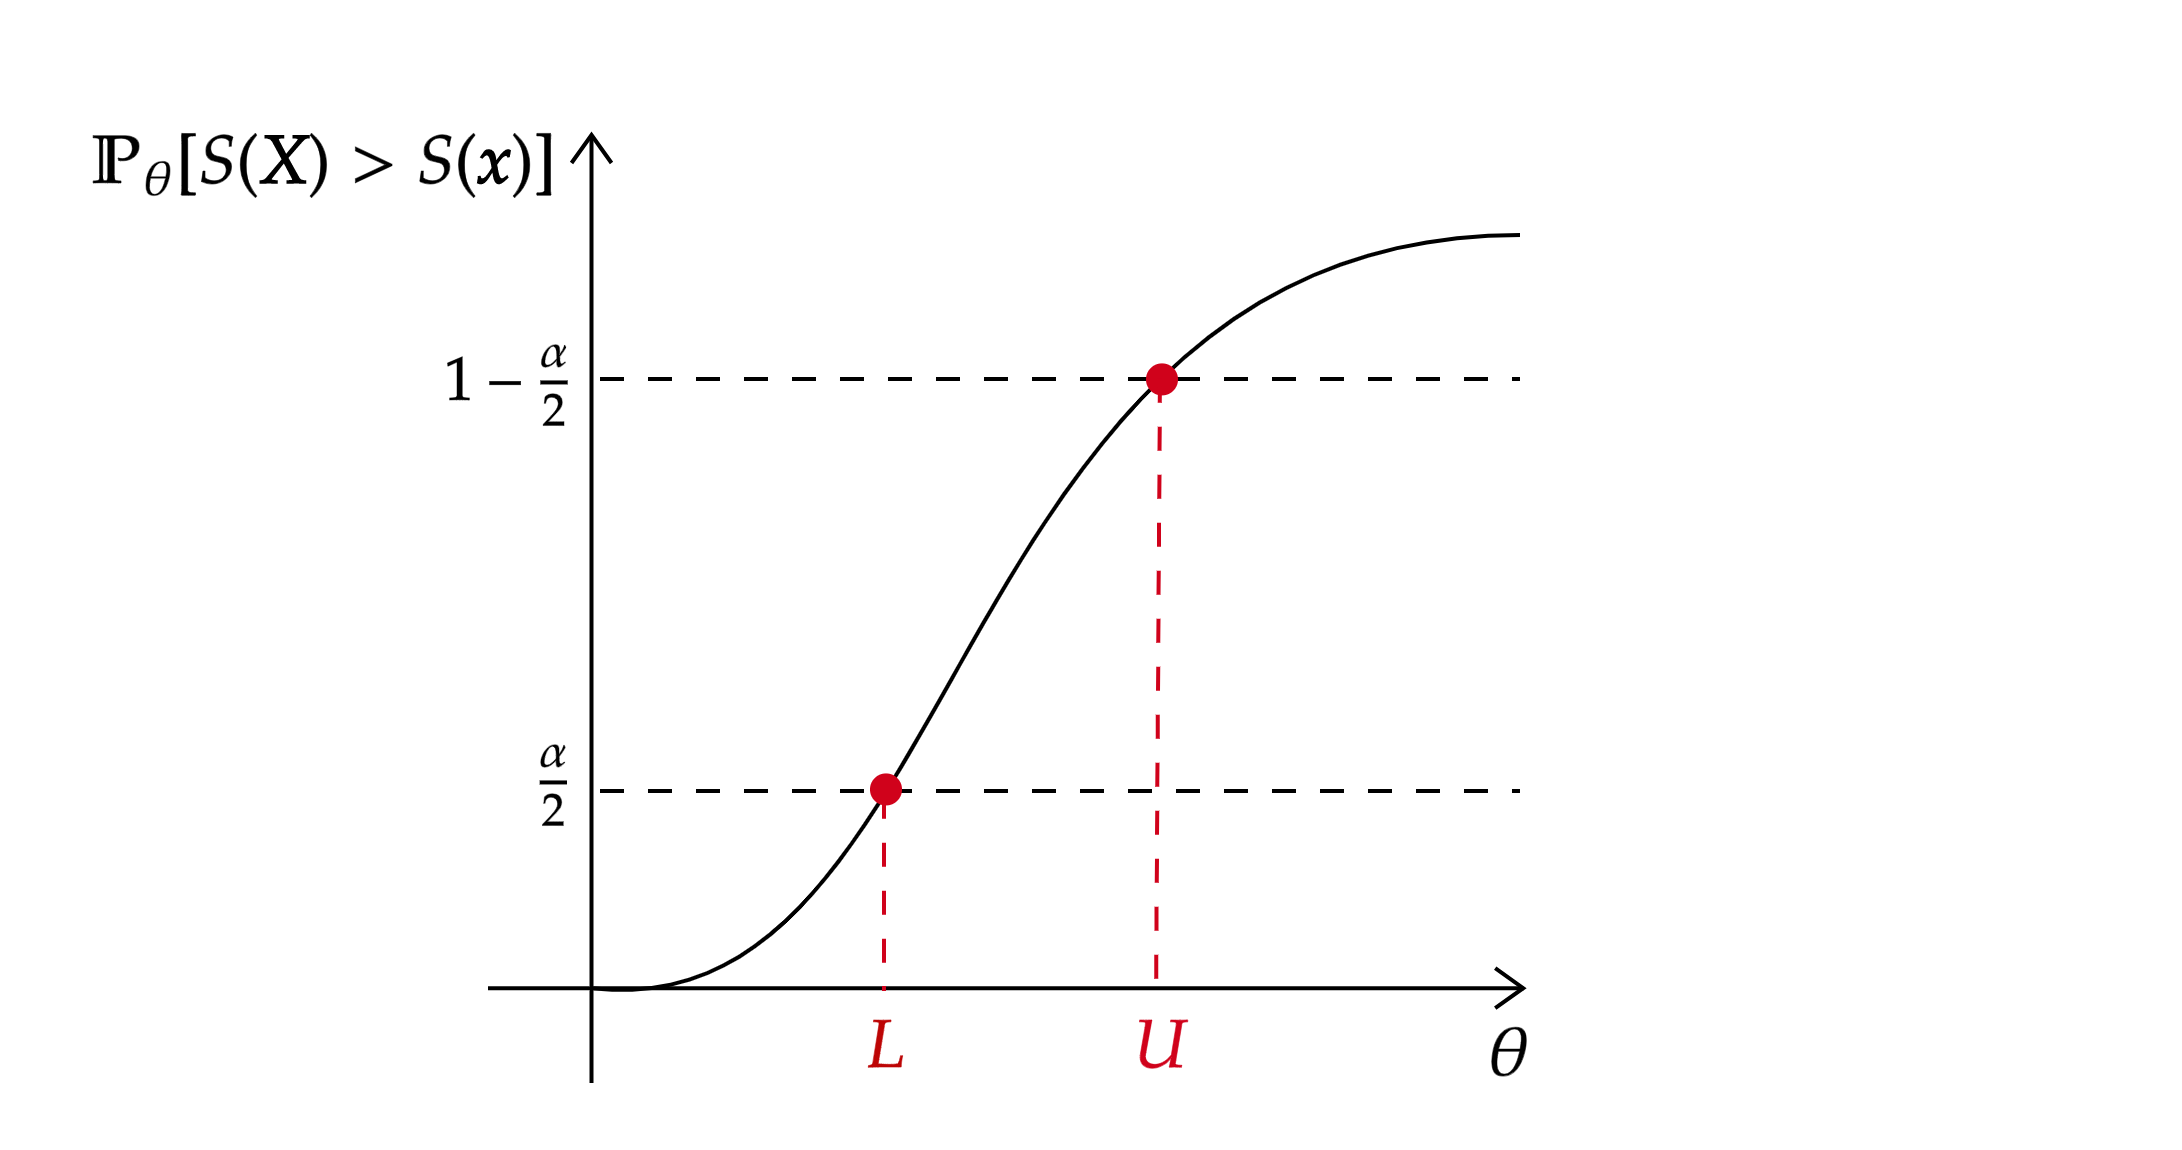
\includegraphics[width=\linewidth]{figures/inversion-diagram.png}
    \caption{The confidence interval - hypothesis test duality. The $100(1-\alpha)\%$ confidence interval for $\theta$, denoted by $[L, U]$, is equivalent to the set of possible values for $\theta$ such that the test statistic $S(\bm{X})$ is in the acceptance region for the null hypothesis. This is only true subject to a stochastically increasing in $\theta$ assumption.}
    \label{fig:inversion_diagram}
\end{figure}

Returning to the simulated-inversion (SI) estimator proposed by \citet{Huang2019}, consider a data generation process following model $M$, which may or may not account for measurement error. The goal is to estimate $\PP_\theta\left\{S(\bm{X}) > S(\bm{x})\right\}$ by simulation, and then construct confidence intervals by inversion. These two steps are described below:

\begin{enumerate}
    \item \textbf{Simulation}: Suppose we have a given dataset $\bm{x} = [x_1, x_2, \dots, x_n]^\top$ and a known set of $r$ potential values for the true extinction time $\bm{\theta} = [\theta_1, \theta_2, \dots, \theta_r]^\top$. Then, for each potential value $\theta_i$, simulate a pseudo dataset $\bm{x}^*_i$ from the model $M$ specified by $\theta_i$ and take a sample statistic $S^*_i$ from the pseudo dataset. Thus, for a given dataset of $n$ observations and a set of $r$ potential values for $\theta$, a set of $r$ simulated statistics $\bm{S}^*$ can be obtained.
    \item \textbf{Inversion}: An estimate for $\PP_\theta\left\{S(\bm{X}) > S(\bm{x})\right\}$ is constructed by regressing the indicator $\mathbbm{1}\left\{ S(\bm{X}^*_i) > S(\bm{x}^*_i) \right\}$ against $\theta_i$ for all $i \in \left\{ 1, \dots, r \right\}$. Finally, $\theta$ can be estimated by inverting the estimated curve.
\end{enumerate}

This method of extinction estimation is very general, as it only requires that the statistic $S(\bm{X})$ is stochastically increasing in $\theta$. It also imposes no other restrictions on the statistic $S(\bm{X})$ used to construct the interval, and imposes no restrictions on the simulation model used to estimate $\PP_\theta\left\{S(\bm{X}) > S(\bm{x})\right\}$, meaning it can be applied regardless of the complexity of the data generation model. Thus, the SI estimator could be used for broader settings beyond the uniform distribution assumption, and could readily account for the presence of measurement errors. For example, Huang suggests the Simulated Inversion - Uniform Gaussian Minimum (SI-UGM) estimator which uses the simulated inversion estimator with the minimum statistic and simulates fossils as uniformly distributed with Gaussian measurement errors \citep{Huang2019}. 

That being said, there are some disadvantages to the SI estimator. Since the true extinction time is unknown, the interval of potential values for $\theta$ must necessarily be wide (and even wider where confidence intervals need to be constructed), which can negatively impact the required computation time for estimating extinction times. In the inversion step, \citet{Huang2019} estimated $\PP_\theta\left\{S(\bm{X}) > S(\bm{x})\right\}$ using a regression method that is not necessarily monotonic, and so this method could be improved by enforcing monotonicity, a conclusion supported by work done by \citet{King2020}.

\chapter{Proposed Methods}\label{chap: proposed-methods}

In this chapter, we propose two new methods for estimating any sample quantile $\theta_q$ of the true extinction date, given a set of fossils. Both of these methods use test-statistic inversion: we first describe a novel approach called MINMI, which directly inverts a minimum statistic to estimate a quantile; then we describe SI-RM, an application of the the Robbins-Monro process, which can be considered a stochastic approximation extension of the simulated inversion estimator. 

\section{Minimum-Statistic Inversion (MINMI) Estimator}\label{new-method}

The MINMI\footnote{The name MINMI is a reference to \textit{Minmi Paravertebra}, a species of ankylosaur (or armoured dinosaur). Notably, \textit{Minmi} is the only known genus of ankylosaur from Australia, and was found in north-central Queensland \cite{Carpenter2001}. They were herbivores!} estimator assumes fossil recovery is uniformly distributed and that the distribution of measurement errors is known with constant variance. Then, using these assumptions, we are able to directly construct a quantile estimator by inversion.

\subsection{No Measurement Error Scenario}

Under the \hyperref[model: no-measurement-error]{$\delta$-model} proposed in \autoref{section: delta-model}, our fossil ages $X_i$ are uniform over $[\theta, K]$. Hence, we can compute the quantile function of the test-statistic $S(\bm{X})$ directly. Let the test statistic $S(\bm{X})$ be the MLE, the minimum statistic, and let $m$ denote the observed minimum value of $S(\bm{X})$:
\[
    \PP_\theta (S(\bm{X}) \geq m) = \prod_{i=1}^n \PP_\theta (X_i \geq m) = \left[ \PP_\theta (X_i \geq m) \right]^n = \left( \frac{K - m}{K - \theta} \right)^n
\]
\clearpage
Applying test-statistic inversion as per \autoref{eq: inversion}, we have
\begin{align*}\label{eq:minmi-no-measurement-error}
    q &= \PP_{\hat{\theta}_q}(S(\bm{X} \geq m) = \left( \frac{K - m}{K - \hat{\theta}_q} \right)^n \\
    \therefore \hat{\theta}_q &= K - q^{-1/n} (K-m) \numberthis
\end{align*}

where $\hat\theta_q$ is the MINMI estimate of $\theta_q$, such that $\PP_{\theta_q} (S(\bm{X}) \geq m) = q$.

\subsection{Measurement Error Scenario}

Let us next consider a scenario where measurement error is substantial. Under the \hyperref[model: measurement-error]{$\varepsilon$-model} proposed in \autoref{section: varepsilon-model}, where measurement error is assumed to be substantial, we have conditionally uniform fossil ages.

Consider the joint density of $(X, \varepsilon)$:
\[
    f_{X, \varepsilon} ( x , \varepsilon) = c f_{X | \varepsilon} ( x | \varepsilon=e) f(e)
\] where $x > \theta$, $x+e \leq K$, and $c$ is a normalising constant. Rearranging to find $c$:
\begin{align*}
    c^{-1}
        &= \int_{-\infty}^{K-\theta} \int_{\theta}^{K-e} f_{X | \varepsilon} ( x | \varepsilon=e) f(e) dx de\\
        &= \int_{-\infty}^{K-\theta} f(e) de \\
    \therefore c^{-1} &= F(K - \theta)
\end{align*}
where $F(y)=\int_{-\infty}^{y} f(e) de$ is the CDF of the measurement error.

Thus our joint density function is given by
\begin{align*}
    f_{X, \varepsilon} ( x , \varepsilon)
        =& [F(K - \theta)]^{-1} f_{X | \varepsilon} ( x | \varepsilon=e) f(e) \\
        =& [F(K - \theta)]^{-1} \frac{1}{K - e - \theta} f(e)
\end{align*}
since $X_i | \varepsilon_i \sim \mathcal{U}(\theta, K-\varepsilon_i)$. 

From this, we can geometrically identify our region of interest as shown by the shaded region of \autoref{fig: minmi_integral}.
\begin{figure}[ht]
    \centering
    \includesvg[inkscapelatex=false,width=0.85\linewidth]{figures/plot_minmi_joint_density.svg}
    \caption{Sketch of the region of the joint density $(X, \varepsilon)$, indicated by the shaded area bounded by  $X+\varepsilon = K$ and $X + \varepsilon = w$, where $X \in [\theta, K]$ and $\varepsilon <= K-\theta$.}
    \label{fig: minmi_integral}
\end{figure}

Hence, we can find $\PP_\theta ( X + \varepsilon \geq w)$ for some value $w$. \begin{align*}
    \PP_\theta ( X + \varepsilon \geq w)
        =& 1 - \PP_\theta ( X + \varepsilon < w) \\
        =& 1 - \int_{-\infty}^{w-\theta} \int_{\theta}^{w-e} f_{X, \varepsilon}(x, e) dx de \quad \text{by inspection} \\
        =& 1 - \int_{-\infty}^{w-\theta} \int_{\theta}^{w-e} \frac{1}{K - \theta - e} \frac{1}{F (K - \theta)} f(e) dx de \\
        =& 1 - \frac{1}{F (K-\theta)} \int_{-\infty}^{w-\theta} \frac{w - \theta - e }{K - \theta - e} f(e) de \\
    \therefore \PP_\theta ( X + \varepsilon \geq w) =& 1 - \frac{F(w-\theta)}{F(K - \theta)} \psi(\theta; w) \numberthis \label{eqn:minmi}
\end{align*}
where $\psi(\theta; w) =  \int^{w-\theta}_{-\infty} \frac{w - e - \theta}{K - e - \theta) } \frac{f(e)}{F(w-\theta)} de$.

As before, we let our statistic $S(\bm{W})$ be the minimum statistic, $m$ be the observed minimum, and take $\theta_q$ such that $\PP_{\theta_q} (S(\bm{W}) \geq m) = q$:
\begin{align*}
    \PP_{\theta_q} (S(\bm{W}) \geq m)
      &= \prod_{i=1}^n \PP_{\theta_q} (X_{i} + \varepsilon_i \geq m) \\
    \implies q &= \left[ 1 - \frac{F(m-\theta_q)}{F(K - \theta_q)} \psi(\theta_q; m)  \right]^n \\
    q^{\frac{1}{n}} &= 1 - \frac{F(m-\theta_q)}{F(K - \theta_q)} \psi(\theta_q; m) \numberthis \label{eqn: minmi-ee}
\end{align*}
The MINMI estimator $\hat\theta_q$ can be found using inversion by solving the above \autoref{eqn: minmi-ee} for $\theta_q = \hat\theta_q$. However, since $\psi$ does not simplify in general, we propose approximate it with a Monte Carlo integral using $B$ Monte Carlo samples from $f(e)$, resulting in the below MINMI estimating equation:
\begin{align*}
    q^{\frac{1}{n}} &= 1 - \frac{F(m - \theta_q)}{F(K - \theta_q)} \hat\psi_B(\theta_q; m); &\hat\psi_B(\theta_q; m) =  \frac{1}{B} \sum_{b=1}^B \frac{m-e_b-\hat\theta_q}{K-e_b-\theta_q} \numberthis \label{eqn: minmi-ee-mc}
\end{align*} where $e_b$ are drawn from $f(e_b)$ truncated at $m-\hat\theta_q$

\subsection{Stochastically Increasing Property}\label{subsec: stochastically-increasing}

Generating confidence intervals by inversion is conditional on $\PP_{\theta} (S(\bm{W}) \geq m)$ being stochastically increasing in $\theta$. Although we were unable to show theoretically that this condition is true in general, we expect that it will be in most practical instances, and have been able to show this numerically under a range of parameter settings. We have been able to show that $\PP_{\theta_q} (S(\bm{W}) \geq m)$ is stochastically increasing under two assumptions, as below.
\begin{restatable}{theorem}{MinmiStochIncr}\label{theorem: stoch-increasing}
    Under the \hyperref[model: measurement-error]{$\varepsilon$-model} specified in \autoref{section: varepsilon-model}, if the following assumptions are satisfied:
    \begin{enumerate}
        \item The density function $f$ is symmetric and uni-modal about mean 0.
        \item $f(2|m-\theta|) > f(K-\theta) \left(2 + \frac{K-\theta}{|m-\theta|} \right)$
    \end{enumerate}
    Then $\PP_{\theta} (S(\bm{W}) \geq m)$ is stochastically increasing in $\theta$.
\end{restatable}

The proof of \autoref{theorem: stoch-increasing} is provided in \autoref{apx:minmi-stoch-incr-proof}.

Assumption 1 in \autoref{theorem: stoch-increasing} is clearly satisfied when we use a normal distribution to simulate measurement error, as we do in this thesis. Assumption 2 is not true at all values of $\theta$ (for example, if we were to choose $\theta$ to be arbitrarily close to $K$). But such values of $\theta$ are not plausible -- recall that $K$ and $\theta$ are the endpoints of the time interval under consideration, and $m$ is the most recently observed fossil. Hence $m$ we expect to be much closer to $\theta$ than to $K$ in settings of practical interest. Further, $K-\theta$ will typically be very large relative to measurement error, meaning that $f(K-\theta)$ will be very small, relative to $f(2|m-\theta|)$.

\subsection{Selecting the number of Monte Carlo Samples}\label{subsec:minmi-mce-var}

As the number of Monte Carlo samples increases, the variance of the MINMI estimator can be expected to decrease at the cost of greater computation: however, we would like to determine a way to obtain a ``good" value for $B$.

Using the delta method, we found the limiting distribution of $\sqrt{B}(\hat\theta_q - \theta_q)$ (a full derivation of is given in \autoref{apx:minmi-asymptotics-proof}):
\begin{restatable}{theorem}{ChooseMinmiB}\label{theorem: delta-method-variance}
    Under the \hyperref[model: measurement-error]{$\varepsilon$-model}, the limiting distribution of the MINMI estimator $\hat\theta_q$ is approximately normal as $B \rightarrow \infty$
    \[
        \sqrt{B}(\hat\theta_q - \theta_q) \stackrel{D}{\rightarrow} \cN \left(0, \sigma^2_{\psi(\theta_q)} \left[ \frac{F(m-\theta_q)}{F(K-\theta_q)\hat{u}^\prime(\theta_q)} \right]^2 \right)
    \] where $\sigma^2_{\psi(\theta_q)} = \Var\left(\psi(\theta_q)\right)$, $\psi(\theta) =  \int^{m-\theta}_{-\infty} \frac{m - e - \theta}{K - e - \theta) } \frac{f(e)}{F(w-\theta)} de$, $F(e)$ is the CDF of $\varepsilon$, and $\hat{u}(\theta) = \frac{F(m-\theta)}{F(K-\theta)} \hat{\psi}(\theta) - 1 + q^{1/n}$.
\end{restatable}

We were able to verify this result numerically, and observed the variance estimated by the delta method in \autoref{theorem: delta-method-variance} to be accurate to within 15\% for $B > 100$. This was done by comparing the delta method variance estimate to the sample variance of 250 MINMI estimates, repeating this process for values of B up to 3500. We verified this result for both the upper and lower endpoints of a central $95\%$ confidence interval at different values of $B$.
\begin{figure}[ht]
    \centering
    \includesvg[inkscapelatex=false, width=0.7\linewidth]{figures/minmi-delta-method_variance.svg}
    \caption{Percentage difference of the variance estimated by the delta method and the variance found numerically as $B$ increases. Note that the x-axis is on a $\log$ scale. The area shaded in green represents the region where the variance is accurate within 15\%, which we observed for $B > 100$. The dashed line indicates $B=100$.}
    \label{fig: minmi-delta-method-variance}
\end{figure}

In practice, we are interested in the value of $B$ that results in an estimator with ``low" variance. Rearranging the variance expression in \autoref{theorem: delta-method-variance}:
\begin{align*}
    \Var(\hat\theta_q) &\approx \frac{1}{B}\sigma^2_{\psi(\theta_q)} \left[ \frac{F(m-\theta_q)}{F(K-\theta_q)\hat{u}^\prime(\theta_q)} \right]^2 \\
    \implies B &\approx \frac{1}{\Var(\hat\theta_q)}\sigma^2_{\psi(\theta_q)} \left[ \frac{F(m-\theta_q)}{F(K-\theta_q)\hat{u}^\prime(\theta_q)} \right]^2
\end{align*}
Suppose we would like estimates with Monte Carlo error variance that is no larger than some small value $A$. Let $B^*$ denote the number of Monte Carlo samples required to achieve this. Then,
\begin{equation}\label{eqn:minmi-optimal-b}
    B^* \approx \frac{1}{A}\sigma^2_{\psi(\theta_q)} \left[ \frac{F(m-\theta_q)}{F(K-\theta_q)\hat{u}^\prime(\theta_q)} \right]^2
\end{equation}
Note that we must approximate $\theta_q$ and $\sigma^2_{\psi(\theta_q)}$ as their true values are unknown. For our purposes, pilot estimates for each will suffice: for instance, $\theta_q$ can be estimated using the MINMI estimator under the $\delta$-model as per \autoref{eq:minmi-no-measurement-error}, and a Monte Carlo estimate of $\sigma^2_{\psi(\theta_q)}$ can be obtained using some pilot number of Monte Carlo samples, such as $B=100$. For this thesis, we aimed to find estimates with Monte Carlo error variance no more than 20\% of our assumed measurement error variation, setting $A = 0.2*\sigma^2$.

\section{Simulated Inversion - Robbins Monro Process (SI-RM)}

We now propose applying the Robbins-Monro (RM) process to the estimation of extinction times, motivated by an application of the RM process to construct confidence intervals by \citet{Garthwaite1992}. We relate this to the simulated inversion estimator proposed by \citet{Huang2019} and apply it to estimating extinction times. Although the RM process has not yet been used to search for extinction times or endpoints of confidence intervals in palaeobiology, it is a generally well used technique in other spaces \cite{Carpenter1999, Fisher2020, Fu2015}.

\subsection{The Robbins-Monro Process}

The RM process is a stochastic approximation algorithm originally designed to solve various root-finding problems. It was later adapted to a specific root-finding problem of the form \cite{Fu2015} \[
M(\theta) \overset{\text{def}}{=} \E_\theta H(\bm{W}) = \beta
\] where $H(\bm{W})$ is some function of random variables $\bm{W}$ and $\beta \in \R$. The objective of the RM process is to find a sequence $\{\theta_n\}$ that converges to a unique (local) optimum $\theta^*$ by using the recursion \cite{LlyodBotev2015}
\[ \theta_{i+1} = \theta_i - c_i \Big( H(\bm{W}_i) - \beta \Big) \]
where $c_i > 0$ is the step size. \citet{RobbinsMonro1951} showed that, under weak regularity conditions, this recursion converges in mean square to the optimum $\theta^*$. However, the step sizes $c_n$ must decrease according to conditions $\sum_nc_n^2 < \infty$ and $\sum_n c_n = \infty$.

\subsection{The SI-RM Estimator}

We propose an inversion-based method for constructing central $100(1-\alpha)\%$ confidence intervals for $\theta$, applying the implementation of the RM process developed by \citet{Garthwaite1992}. They adapted the original scheme by letting $M(\theta) = \PP_\theta(S(\bm{W} > S(\bm{w}))$ and $\beta = \alpha/2$ (for the lower endpoint of the confidence interval, and $1-\alpha/2$ for the upper endpoint) where $S(\bm{w})$ is a point estimator of $\theta$. This scheme is described for the lower endpoint as follows:
\begin{align*}
    M(\theta) \overset{\text{def}}{=} \PP(S(\bm{W} > S(\bm{w})) = \alpha/2
\end{align*}

\citet{Garthwaite1992} designed this method to construct confidence intervals assuming that a point estimate (for instance, the maximum likelihood estimator) can be easily obtained, although in principle any statistic could be used if it is stochastically increasing in $\theta$, and as such we use $S(\bm{w})$ as previously. Next, let $\hat\theta_{q; i}$ be the estimate of $\theta_q$ at step $i$ of the RM process, for the $q$\textsuperscript{th} quantile. At each step of the process, generate a resample $\bm{w}^* = [w_1^*, \dots, w_n^*]$ by setting $\theta = \hat\theta_{q; i}$. Then, the next estimate $\hat\theta_{q; i+1}$ can be found by the recursion
\begin{equation}\label{eqn: SIRM-recursion}
    \hat\theta_{q; i+1} = \hat\theta_{q; i} - c/i \left( \mathbb{I}\left[S(\bm{w^*}) > S(\bm{w})\right] - q \right)
\end{equation}
where $c$ is a predetermined step length constant and $\mathbb{I}$ is the indicator function.

The resample step, where we simulate new data according to our simulation model by setting $\theta = \hat\theta_{q; i}$, is similar to the simulated inversion estimator proposed by \citet{Huang2019}. As such, the application of the RM process can be thought of as a variation of the simulated-inversion estimator, where stochastic approximation is used to converge to an optimal estimate of $\theta_q$.

The recursion in \autoref{eqn: SIRM-recursion} must be adapted for the uniformity assumption in Models \ref{model: no-measurement-error} and \ref{model: measurement-error}, since $\theta_q$ must be positive and less than $K$. We propose recursing on a transformation of $\hat\theta_{q; i}$, to allow step sizes to still be defined on $\R$ while enforcing $\hat\theta_{q;i} < K$. Let $\eta$ be the following transformation:\begin{equation}
    \eta(\theta) = K -\ln(K-\theta)
\end{equation}
Hence, the recursion in \autoref{eqn: SIRM-recursion} becomes:
\begin{equation}
    \hat\eta_{q; i+1} = \hat\eta_{q; i} - c/i \left( \mathbb{I}\left[S(\bm{w^*}) > S(\bm{w})\right] - q \right)
\end{equation}
where $c_\eta$ denotes predefined step lengths that are on the same scale as $\eta$.

Estimates based on the RM process are clearly advantageous when the function $M(\theta)$ is unknown or too complex to be directly inverted. An example of this is if the uniformity assumption is relaxed, as depending on the distribution of the fossils, $M(\theta)$ may potentially be too complex to apply a method similar to the MINMI estimator. 

However, there are still some disadvantages to the SI-RM estimator. The flexibility of this method means we may expect it to be slower than MINMI, which exploits our knowledge of the form of the quantile function $P_{\theta_q}(S(\bm{W})>S(\bm{w}))$ to directly find an estimate. This will be explored by simulation in the next chapter. Moreover, the flexibility also means the method must be \textit{tuned} for each problem on a case-by-case basis, as choices of step size, starting values, and stopping criteria all significantly impact the exactness of estimates.

\subsection{Choice of Step Size}

The choice of $c$ has a significant impact on the performance of the RM process: too large, and the algorithm may oscillate back and forth without approaching the optimum; too small (relative to the magnitude of the gradient), and the iterates may never move, preventing convergence.

The optimal step length (let this be $c^*$) is dependent on $M^\prime(\theta)$ \cite{LlyodBotev2015}, which is typically unknown. As such, \citet{Garthwaite1992} proposed an \textit{adaptive} step length where $c_i$ is proportional to the distance between the point estimate $\hat\theta(\bm{y})$ and the current estimate $\theta_{q; i}$:\begin{equation} c_i = \begin{cases}
    k\left(\theta_{q; i} - \hat\theta(\bm{y}) \right) &\text{if $q \geq 0.5$} \\
    k\left(\hat\theta(\bm{y}) - \theta_{q; i}\right) &\text{if $q < 0.5$}
\end{cases}
\end{equation}
where $k$ is a proportionality constant dependent on the distribution of $S(\bm{w})$.

In the absence of better information, \citet{Garthwaite1992} set the step length proportionality constant $k$ to twice the optimal value for the normal distribution: \[
k = 2/\left[z_q \phi(z_q) \right]
\]
The recommendation to double the optimal value for the normal distribution comes because the cost (in terms of impact to the variance) of underestimating $c^*$ is greater than the cost of overestimating it -- specifically, the variance of $\hat\theta_q$ can increase significantly when step sizes are too small.

However, \citet{LlyodBotev2015} found that the above step length proposed by \citet{Garthwaite1992} leads to variances that are 20-30\% greater than the lower bound of the RM variance. Hence, although we will use the adaptive step size scheme in the experiments in subsequent chapters, we recognise this is an area where improvements can potentially be made.

\subsection{Choice of Starting Values}

The starting values used to initiate the RM process also affect convergence -- if initial estimates are not in the neighbourhood of the true value then it may be difficult to converge quickly to the optimum. As a result, \citet{Garthwaite1992} suggested some heuristics for selecting appropriate starting values for the RM process.

They propose the ``percentile method" for selecting starting points, proceeding with the process as though these starting points were reached after $m$ steps. For a $100(1-\alpha/2)\%$ confidence interval, starting values are found by first generating $(4-\alpha)/\alpha$ resamples with $\theta = S(\bm{w})$. The starting values for the upper and lower endpoints are then provided by the second largest and second smallest resamples, respectively.

The number of steps to skip, $m$, is chosen as
\[
    m = \min \left\{ 50, 0.3(4-\alpha)/\alpha \right\}
\]
Although the Robbins-Monro process is robust to the choice of starting values, good starting values improve the rate of convergence. Moreover, step sizes tend to be disproportionately large early on in the search. Hence, if starting estimates are not in the neighbourhood of the true value then the process may be sent far away and convergence may take significantly longer--- see \autoref{fig:SI-RM-starting-values}.
\begin{figure}[ht]
    \centering
    \includesvg[inkscapelatex=false, width=\linewidth]{figures/SI-RM-starting-estimate-convergence.svg}
    \caption{Left: SI-RM searches for the lower endpoint of a 95\% confidence interval. Right: SI-RM searches for the upper endpoint. \textcolor{red}{Red} is the search with starting values chosen by Garthwaite \& Buckland's percentile method \cite{Garthwaite1992}. Each line is a separate RM process performed on the same simulated dataset with different starting values. Note that the RM process converges to similar estimates regardless of the starting value, with the only difference being convergence speed. If starting estimates are too far away, estimates may be ``sent" too far away and substantially impact convergence.}
    \label{fig:SI-RM-starting-values}
\end{figure}

\subsection{Selecting Stopping Criteria}\label{subsec:si-rm-stopping-criteria}

The standard error of estimates obtained by the SI-RM process naturally reduces as the number of steps increases at the cost of computation time. We would like to stop the process once our estimates have variance that is below a certain value. However, there is currently no universal stopping criteria, since we are unable to approximate the expected variance at the $i$\textsuperscript{th} step of the RM process. 
% To determine a stopping rule, we can approximate the SI-RM estimator's variance at each iteration; if the approximate variance is below a predetermined threshold variance, the process is terminated. Otherwise, the process continues until some maximum number of iterations $i_\text{max}$ is reached.

Consider the limiting variance of the $(i+1)$\textsuperscript{th} estimate, which can be found using the delta method \cite{Garthwaite1992}
\[
    \Var(\hat\theta_{q; i+1}) = \frac{\alpha/2 (1-\alpha/2) c^2}{i(2gc-1)}, \quad g = \left[ \frac{d}{d\hat\theta_q}M(\hat\theta_q) \right]_{\hat\theta_q = \theta_q}
\]
In practice, neither $\frac{d}{d\theta}M(\theta)$ or $\theta_q$ are known, so $\Var(\hat\theta_{q; i+1})$ cannot be calculated. Currently there is no universal stopping criteria for the RM process; \citet{Garthwaite1992} proposed a manual approach by inspection, allowing the RM process to iterate for some time, pausing and inspecting for convergence, then restarting if not converged. In our simulation studies, we will use the estimated quantile function from the SI estimator proposed by \citet{Huang2019}, estimating $\frac{d}{d\theta}M(\theta)$ by symmetric finite difference \cite{Fu2015} for the purpose of illustrating the potential of this method.

\chapter{Simulation Studies}\label{chap: simulation-experiments}

In this chapter we study the performance of the existing and proposed methods for estimating extinction times and constructing confidence intervals, using synthetic datasets generated under known conditions. To investigate the performance of these methods with increasing measurement error variation, we repeated the experiments by multiplying the measurement errors by factors of 0 (representing the no measurement error scenario), $0.5$, 1, and 2 (representing a high measurement error scenario). For each ``error factor", we generated 1000 synthetic datasets.

Denote the $i\textsuperscript{th}$ sample of the $j\textsuperscript{th}$ synthetic dataset by $W_{i, j} = X_{i, j} + \varepsilon_{i, j}$, where each fossil is conditionally uniform on a corresponding measurement error and is distributed on the interval $\left[ \theta_0, K - \varepsilon_{i,j} \right]$. For these trials, we set the true extinction date $\theta_0 = 10,000$, and set the known upper bound $K = 20,000$ as the speciation date. Assume that the measurement errors are normally distributed with mean 0 and constant variance $\sigma^2$, which is arbitrarily selected according to a real fossil dataset: \[
W_{i, j} = X_{i, j} + \varepsilon_{i, j}; \quad X_{i, j} \sim \mathcal{U}(\theta_0, K - \varepsilon_{i, j}), \quad \varepsilon_{i, j} \sim \cN(0, \sigma^2)
\] for all $i \in \{1, 2, \dots, 20\}$ and $j \in \{1, 2, \dots, 1000\}$ where $\theta_0 = 10000$ and $K = 20000$.

\section{Point Estimates}

In these experiments, we compared the performance of the different methods' point estimates of extinction times across four metrics: the mean squared error, bias, variance, and average run time. We considered the following seven estimators: MLE, Bias-Adjusted MLE (BA-MLE), the Strauss estimator, GRIWM, SI-UGM, and MINMI. For the SI-UGM, SI-RM, and MINMI estimators, point estimates were obtained by estimating the median $\hat\theta_{q=0.5}$. Note that we exclude the SI-RM estimator in these experiments as it estimates quantiles relative to a given point estimate: hence point estimates produced by SI-RM would be equivalent to the MLE.

We first considered the \textbf{no-measurement error scenario }in order to form a baseline comparison against the MLE, BA-MLE, and Strauss estimators which do not account for measurement error. The best methods were the bias adjusted MLE and the Strauss estimator, which were both designed to be statistically optimal under uniformity assumptions and no measurement error. These two estimators show little to no bias with the best MSE out of the seven methods (\autoref{tab:table-sim-exp-point-error0}).
 
Finally, although MINMI, GRIWM, and SI-UGM produced relatively low MSE estimates, they remained relatively \textbf{positively biased}. This is because these three estimates use a median-based estimate: the sampling error in the data naturally means a median-based estimate would be biased upwards, as estimates would be skewed upwards towards the data rather than being centered on the true value. We also note that the MINMI, GRIWM, and SI-UGM estimators had relatively low variance compared to the BA-MLE and Strauss estimators.
\begin{table}[ht]
    \centering
    \caption{Point estimator performance, ordered by MSE (error = $0*\sigma$)}
    
\begin{tabular}{lrrrr}
\toprule
\multicolumn{1}{c}{Method} & \multicolumn{1}{c}{MSE} & \multicolumn{1}{c}{Bias} & \multicolumn{1}{c}{Variance} & \multicolumn{1}{c}{Average Runtime} \\
\cmidrule(l{3pt}r{3pt}){1-1} \cmidrule(l{3pt}r{3pt}){2-2} \cmidrule(l{3pt}r{3pt}){3-3} \cmidrule(l{3pt}r{3pt}){4-4} \cmidrule(l{3pt}r{3pt}){5-5}
 & (000's years) & (years) & (000's years) & (seconds)\\
\midrule
STRAUSS & 1186 & 534 & 1127 & 0.00002\\
BA-MLE & 1202 & 545 & 1130 & 0.00050\\
MINMI & 1339 & 678 & 1099 & 0.00001\\
GRIWM & 1345 & 684 & 1098 & 2.46991\\
SI-UGM & 1366 & 710 & 1078 & 2.61586\\
\addlinespace
GB-RM & 1811 & 995 & 1025 & 0.03711\\
MLE & 1811 & 995 & 1025 & 0.00002\\
\bottomrule
\end{tabular}

    \label{tab:table-sim-exp-point-error0}
\end{table}

We then moved on to the various estimators' performances across various magnitudes of measurement error variance. Looking at the ``expected" scenario shown in \autoref{tab:table-sim-exp-point-error1}, where we did not modify the variance of the measurement error $\sigma$, we see these results are fairly consistent with the no measurement error scenario, the only exception being the performance of the corrected version of GRIWM. The corrected version of GRIWM produced point estimates with the \textbf{lowest MSE} in a measurement error scenario with the second least amount of bias out of the 8 methods. This can be attributed to the changes we proposed, where the threshold probability $p_t$ was set to 0.5 instead of $0.05$ (resulting in a median-based estimate, similar to SI-UGM and MINMI) and the expression for the recovery rate $\lambda$ was bias-adjusted.
\begin{table}[ht]
    \centering
    \caption{Point estimator performance, ordered by MSE (error = $1*\sigma$)}
    
\begin{tabular}{lrrrr}
\toprule
\multicolumn{1}{c}{Method} & \multicolumn{1}{c}{MSE} & \multicolumn{1}{c}{Bias} & \multicolumn{1}{c}{Variance} & \multicolumn{1}{c}{Average Runtime} \\
\cmidrule(l{3pt}r{3pt}){1-1} \cmidrule(l{3pt}r{3pt}){2-2} \cmidrule(l{3pt}r{3pt}){3-3} \cmidrule(l{3pt}r{3pt}){4-4} \cmidrule(l{3pt}r{3pt}){5-5}
 & (000's years) & (years) & (000's years) & (seconds)\\
\midrule
SI-UGM & 182 & -22 & 226 & 2.05977\\
GRIWM & 184 & -65 & 225 & 2.34895\\
MINMI & 184 & -8 & 229 & 0.00047\\
STRAUSS & 213 & -187 & 223 & 0.00112\\
BA-MLE & 217 & -174 & 234 & 0.00110\\
\addlinespace
GB-RM & 266 & 310 & 212 & 0.03539\\
MLE & 266 & 310 & 212 & 0.00033\\
\bottomrule
\end{tabular}

    \label{tab:table-sim-exp-point-error1}
\end{table}

We also found that these results became less consistent as measurement error increased. As an extreme example, we doubled the amount of measurement error variation and found that the BA-MLE and Strauss estimators ``fell off" in their performance, while the methods that account for measurement error in their estimations became much more accurate. An interesting result was that the \textbf{MLE became more accurate}, likely due to the fact that measurement error is negatively skewed since they cannot be greater than $K-\theta$ (see \autoref{fig: minmi_integral}). This means that as we increase the size of our measurement errors, the observed minimum becomes more likely to be less than $\theta$, which tends to cancel out with the positive bias of the MLE and produce fairly good estimates. Logically, this means the \textbf{MLE's estimates are much more varied}, which we can clearly see in \autoref{tab:table-sim-exp-point-error2} as it has the greatest sample variance.
\begin{table}[ht]
    \centering
    \caption{Point estimator performance, ordered by MSE (error = $2*\sigma$)}
    
\begin{tabular}{lrrrr}
\toprule
\multicolumn{1}{l}{Method} & \multicolumn{1}{c}{MSE} & \multicolumn{1}{c}{Bias} & \multicolumn{1}{c}{Variance} & \multicolumn{1}{c}{Average Runtime} \\
 & (000's years) & (years) & (000's years) & (seconds)\\
\midrule
MINMI & 492 & 27 & 492 & 0.00071\\
SI-UGM & 502 & 65 & 498 & 1.68008\\
GRIWM-BA (q=0.5) & 505 & -278 & 428 & 13.94220\\
MLE & 507 & 254 & 443 & 0.00002\\
SI-RM & 507 & 254 & 443 & 0.05993\\
\addlinespace
BA-MLE & 543 & -234 & 489 & 0.00002\\
Strauss & 554 & -248 & 493 & 0.00002\\
GRIWM (q=0.05) & 2507 & -1408 & 526 & 2.36410\\
\bottomrule
\end{tabular}

    \label{tab:table-sim-exp-point-error2}
\end{table}

In summary, we found that the proposed MINMI estimator produces good point estimates that are somewhat biased due to being based on a median. Our simulation experiments reinforced that the BA-MLE and Strauss estimators are optimal under uniformity assumptions where measurement error is negligible, although they become less reliable and less accurate as the magnitude of measurement error increases. The original implementation of GRIWM consistently performed poorly, producing negatively biased estimates, while the corrections we proposed improved its performance significantly in the measurement error scenarios, albeit at a computational cost. Additional result tables from these experiments have been provided in \autoref{apx:extra-tables-figures}.

\section{Confidence Intervals}

Next, we evaluated the performances of four methods for constructing 95\% confidence intervals for extinction times in terms of their coverage probability, width, and runtime: SI-UGM, MINMI, GB-RM, and GRIWM. The point estimators (MLE, BA-MLE, and Strauss estimators) were excluded from these experiments. For the SI-RM estimator, we again applied the heuristics Garthwaite and Buckland suggested for determining appropriate starting levels and adaptive step sizes.

Across all four levels of measurement error, we found that the SI-UGM, GB-RM, and MINMI estimators all produced comparable coverage probabilities close to 95\% (\autoref{tab:table-sim-exp-coverage}). However, SI-UGM tends to estimate more conservative confidence intervals, as indicated by the slightly higher coverage probabilities compared to GB-RM and MINMI, which gives coverage probabilities within 1\% of the nominal coverage probability. GRIWM consistently had the worst performance, with coverage probabilities of less than 30\%; however, its performance improved marginally as measurement error increased. These results may be explained by the considerably narrower intervals produced by GRIWM (\autoref{tab:table-sim-exp-width}) and the significant negative bias (see \autoref{tab:table-sim-exp-point-error0}).
\begin{table}[ht]
    \centering
    \caption{Confidence Interval Coverage}
    
\begin{tabular}{lllll}
\toprule
\multicolumn{1}{c}{ } & \multicolumn{4}{c}{metric} \\
\cmidrule(l{3pt}r{3pt}){2-5}
Method & 0*$\sigma$ & 1*$\sigma$ & 2*$\sigma$ & 4*$\sigma$\\
\midrule
MINMI & 100.0% & 100.0% & 100.0% & 80.0%\\
SI-UGM & 100.0% & 100.0% & 100.0% & 80.0%\\
GB-RM & 100.0% & 100.0% & 100.0% & 80.0%\\
GRIWM & 60.0% & 80.0% & 60.0% & 0.0%\\
\bottomrule
\end{tabular}

    \label{tab:table-sim-exp-coverage}
\end{table}

Moving on to the confidence interval widths, we found that the MINMI and GB-RM estimators produced confidence intervals that are \textbf{slightly narrower} than those obtained by SI-UGM. The wider intervals of SI-UGM  correlate with the higher coverage probabilities obtained by SI-UGM, as wider intervals would naturally mean the true value for $\theta$ would be more likely to be contained in the  estimated interval. GRIWM's poor performance is once again seen here, as it produces significantly narrower confidence intervals than the other three methods, hence its poor coverage probability.
\begin{table}[ht]
    \centering
    \caption{Confidence Interval Width}
    
\begin{tabular}{lrrrr}
\toprule
\multicolumn{1}{c}{Method} & \multicolumn{4}{c}{Average Width} \\
 & 0*$\sigma$ & 0.5*$\sigma$ & 1*$\sigma$ & 2*$\sigma$\\
\midrule
SI-RM & 2054.55 & 2375.39 & 2500.86 & 2459.19\\
SI-UGM & 1961.14 & 2091.09 & 2964.30 & 2351.53\\
MINMI & 1917.16 & 2077.86 & 2932.73 & 2329.95\\
GRIWM-corrected & 0.00 & 548.08 & 1949.67 & 1047.99\\
GRIWM & 0.00 & 608.33 & 2163.50 & 1162.65\\
\bottomrule
\end{tabular}

    \label{tab:table-sim-exp-width}
\end{table}

Finally, we investigated the computational cost of the methods. We found that the MINMI estimator had the fastest runtime across all measurement error scenarios due to it \textbf{directly estimating} the quantile function, using one set of Monte Carlo samples for all calculations. This is compared to GRIWM, SI-UGM, and SI-RM's procedures that all involve repeatedly sampling from a distribution: for example, SI-UGM simulates $n$ samples from a model for each hypothesised extinction time in $\bm{\theta}$.
\begin{table}[ht]
    \centering
    \caption{Confidence Interval Runtime}
    
\begin{tabular}{lrrrr}
\toprule
\multicolumn{1}{c}{Method} & \multicolumn{4}{c}{Average Runtime} \\
 & 0*$\sigma$ & 0.5*$\sigma$ & 1*$\sigma$ & 2*$\sigma$\\
\midrule
SI-RM & 0.0564 & 0.0607 & 0.0599 & 0.0599\\
SI-UGM & 4.7066 & 2.3306 & 1.6801 & 1.9374\\
MINMI & 0.0000 & 0.0013 & 0.0021 & 0.0014\\
GRIWM-BA (q=0.5) & 13.8988 & 13.8825 & 13.9422 & 13.9010\\
GRIWM (q=0.05) & 2.3355 & 2.3589 & 2.3641 & 18.1072\\
\bottomrule
\end{tabular}

    \label{tab:table-sim-exp-runtime}
\end{table}



\chapter{Application}\label{chap: applications}

In this chapter, we discuss the results of applying the proposed MINMI and SI-RM estimators to real datasets to demonstrate their use to paleobiologists, comparing these results to those of the SI-UGM estimator. Our goal is to see if these methods produce estimates and confidence intervals within expectations, given their performance on synthetic datasets with known conditions.

We applied these three methods to 4 fossil records of megafauna believed to have gone extinct in the Late Pleistocene era/early Holocene period: the steppe bison (\textit{Bison Priscus}), the cave bear (\textit{Ursus spelaeus}), the cave hyena (Crocuta spelaea) and the Eurasian woolly mammoth (\textit{Mammuthus primigenius}). We also investigate the results for the cave bear more closely to place our methods in context of the literature.

Since the speciation and invasion dates of the species are not known, we instead chose a value of $K$ for each dataset representing some upper bound on the observations. In the absence of better information, $K$ was set to the start of the last bin in histograms of the data. Extinction time estimates were then found using the data after excluding observations older than this value of $K$. For instance, the value of $K$ for the cave bear was chosen to be $34,000$ by inspecting the histogram in \autoref{fig:applications-histograms}.

A similar process was used to set the input vector of hypothesised values $\bm{\theta}$ for the SI-UGM estimator, which is assumed to cover the entire interval of possible values for the $95\%$ confidence interval. For example, $\bm{\theta}$ for the cave bear was chosen to be all years between $22,000 - 29,000$ years BP.
\begin{figure}[ht]
    \centering
    \includesvg[inkscapelatex=false, width=\linewidth]{figures/applications-hists.svg}
    \caption{Histograms of the four megafauna species' datasets according to default \texttt{ggplot2} binning. Values of $K$ and $\bm{\theta}$ were chosen by inspection of these histograms. From left to right: the cave bear, cave hyena, Eurasian woolly mammoth, and steppe bison.}
    \label{fig:applications-histograms}
\end{figure}

All three methods produced comparable confidence intervals, with similar widths, ranges, and point estimates. These results further confirm the results from the simulation experiments, as the SI-UGM estimator tended to produce wider confidence intervals for the extinction time. Another observation of note is the width of the intervals, which tend to narrow as the sample sizes increase: the intervals for the Steppe Bison, where $n = 13$, are substantially wider than those for the Eurasian Woolly Mammoth where $n = 194$. This can be interpreted as being due to the availability of more information contributing to more precise estimates, and therefore narrower confidence intervals. 
\begin{figure}[ht]
    \centering
    \includesvg[inkscapelatex=false,width=\linewidth]{figures/applications.svg}
    \caption{Extinction time point estimates and confidence intervals found for each of the four megafauna species. From left to right: the steppe bison, cave bear, cave hyena, and Eurasian woolly mammoth.}
    \label{fig:applications-confidence-intervals}
\end{figure}

\section{Case Study: Cave Bear (\textit{Ursus spelaeus})}

To place our results in context, we consider the cave bear as an example of extinct megafauna from the Pleistocene era. Having disappeared towards the end of the last glacial period, the causes of extinction and precise extinction time has been in debate over the years. In a 2016 study by \citet{Baca2016}, the authors analysed a dataset of over 200 fossil samples of cave bears to construct 95\% confidence intervals for the extinction time, estimating it to have occurred between $26,100 - 24,300$ cal. years before present (BP). The authors also took a more conservative approach, excluding younger dates to obtain an earlier confidence interval of between $27,000 - 26,100$ years BP. These extinction times coincide with the last glacial period which, along with anatomical evidence pointing to a vegetarian diet, suggests their disappearance was largely due to the scarcity of food during the onset of the last glacial period rather than the result of climate change inflicted habitat loss or overhunting from humans \cite{Pacher2009}. 

For this thesis, we estimated extinction times from a dataset of 30 cave bear fossils using the MINMI, SIRM, and SI-UGM methods, constructing confidence intervals that suggested extinction occurring roughly between $29,000 - 27,000$ cal. years BP. These results are somewhat comparable to those obtained by \citet{Baca2016}, as the extinction times belong to the same part of the last glacial period and hence support the same conclusion that changes in the climate from the onset of an ice age reduced the availability of plant life for cave bears to feed upon, triggering their extinction. However, it is clear that the intervals we estimated are substantially wider and more biased in comparison. This can be attributed to the fact that our dataset is both significantly smaller and  more biased in comparison: the smaller sample size results in wider intervals that reflect the increased uncertainty in our estimates, and as \autoref{fig:applications-histograms} shows, the youngest sample in our dataset is dated to approximately $28,000$ year BP, explaining the positive bias in our results. Hence, although the results for the cave bear obtained by our estimation methods may not necessarily reflect the true extinction times due to the quality of our dataset, we believe these results nonetheless demonstrate the performance of the MINMI and SIRM estimators, showing that they contend with existing methods and produce reliable and robust estimates that are consistent with the literature.

\chapter{Conclusions and Future Directions}\label{chap: conclusions}

In this thesis, we proposed two novel applications of test-statistic inversion to estimate extinction times in the fossil record: the Minimum Statistic Inversion (MINMI) estimator and the Simulated Inversion - Robbins Monro Process (SI-RM). We explored these methods under assumptions of uniformly distributed fossils with both negligible measurement error and substantial measurement error, performing simulation studies to explore the performance of the obtained point estimates and confidence intervals in relation to existing methods.

Most previously developed methods assumed uniformity and negligible measurement error, and our methods are a significant advance on this. We further expect that we could extend our methods to arbitrarily distributed fossils and measurement errors, using inversion to make exact inference (under some monotonicity conditions).

In our simulation studies, we showed that the proposed methods produce point estimates that are comparable to existing methods, and can construct confidence intervals with better coverage, more appropriate widths, and faster computation times compared to existing methods such as GRIWM and SI-UGM. In particular, the MINMI estimator needs no tuning to produce 95\% confidence intervals with reliable coverage, an advantage held even as the magnitude of the measurement error uncertainty changed. On the other hand, the confidence intervals estimated by SI-RM had less reliable coverage probabilities, which can be addressed by increasing the number of iterations. However, SI-RM has the benefit of flexibility, as it can be easily adapted to less strict assumptions since the simulation model can be tuned to better fit the true data generating process.

We then applied the MINMI and SI-RM estimators to datasets of megafauna fossils (the steppe bison, cave bear, cave hyena, and Eurasian woolly mammoth) and observed similar results to the simulation studies. We found that the proposed methods generated comparatively wider confidence intervals to reflect the uncertainty around the true extinction time.

A key assumption made throughout this thesis is that fossils are uniformly distributed, and an opportunity going forward is to relax this assumption. Although it is common practice to assume uniformity, there is substantial evidence to suggest this is not valid as we can expect a species to be less abundant closer to speciation and extinction \cite{Lee2010, WangMarshall2016}. As a result, it would be worthwhile to explore the robustness of the proposed methods to alternative models, or adjust their design accordingly. For instance, one approach may be to use recovery rates from other fossil datasets' to estimate the distribution via kernel density estimation. Other suggestions include modelling fossil recovery as sigmoidal or exponentially distributed as per \citet{Bradshaw2012}, or using a ``reflected beta distribution" as per \citet{Wang2016}. However, unlike many existing methods, the proposed estimators are more flexible and can be adapted to alternative models: this is especially true for the SI-RM estimator, as the simulation model simply needs to be adjusted accordingly. On the other hand, although the MINMI estimator can be adapted to a non-uniform model, the quantile function will need to be re-derived as currently this method's advantages are related to the exploitation of the conditionally uniform distribution of fossils.

A common assumption in the literature that has been carried over into this thesis is the independence of measurement error. Since radiocarbon ages are often calibrated using the same calibration curves, it is possible for the measurement errors to be correlated. This is known as a ``curve offset" \cite{Ramsey2010}. In his master's thesis, \citet{King2020} proposed an application of simulated inversion to account for calibration errors. We expect these to work similarly for SI-RM by adapting the simulation model accordingly. On the other hand, more work needs to be explore how the MINMI estimator can account for correlated calibration error.

In addition, it remains to be seen in general that the quantile function under the measurement error scenario (Model \ref{model: measurement-error}) is stochastically increasing in $\theta$, an important condition for the application of test-statistic inversion. Although we were able to numerically verify this condition as well as show it is satisfied under some additional constraints (see \autoref{apx:minmi-stoch-incr-proof}), this remains an area of investigation for the future that may benefit the development of estimation methods based on test-statistic inversion.

Although the performance of our proposed methods is fairly good, a potential area of improvement is the choice of the test-statistic. The MINMI estimator uses the minimum statistic for inversion in the measurement error scenario, which was chosen because it is the MLE under the no-measurement error scenario. A better statistic could potentially be found, which may further improve estimates although the degree of improvement is uncertain. This is also true for the SI-RM estimator, which uses the test-statistic to select adaptive step lengths.

The SI-RM estimator may be improved across several aspects, such as the choice of step-length constant and stopping criteria. The SI-RM estimator uses the recommendations made by \citet{Garthwaite1992}, who proposed a heuristic that gives asymptotically exact results where the distribution of the point estimate is similar to a normal distribution, which could be further refined: for instance, \citet{LlyodBotev2015} suggested a step-length constant without normality assumptions that could be used to refine the step length constant following a burn-in period. Furthermore, additional work needs to be done to identify appropriate stopping criteria for the RM process, as stopping too early results in poor coverage and incorrect estimates.

In summary, the MINMI and SI-RM estimators proposed in this thesis are competitive alternatives to what currently exists for estimating extinction times. These methods produce comparable point estimates and significantly better confidence intervals compared to existing methods, and can be readily adapted to less strict assumptions which other methods are unable to do. These methods can also be further extended and improved across various areas to estimate extinction times under less convenient assumptions.

Some \texttt{R} code implementing the MINMI and SI-RM estimators has been provided in \autoref{apx:code-minmi} and \autoref{apx:code-si-rm}. Additional scripts and notebooks used for this thesis, such as the simulation studies and application, are available online on GitHub: \url{https://github.com/victorwctsang/Inversion-Extinction-Estimates}

\appendix

\chapter{Proof: Bias of the Maximum Likelihood Estimator}\label{apx:mle-bias-proof}
We would like to prove that under the \hyperref[model: no-measurement-error]{$\delta$-model}, the MLE of $\theta$ has bias $= \frac{K-\theta}{n+1}$.
\begin{proof}
    Given that $X_1, \dots, X_n$ are independent and uniformly distributed on $[\theta, K]$, the CDF is \[
    \PP_\theta(X_i \leq x) = \begin{cases}
                0 & x > K \\
                \frac{x-\theta}{K-\theta} & x \in [\theta, K] \\
                1 & x < \theta
            \end{cases}
    \]
    Now, as shown in \autoref{section:MLE}, the MLE is the first order statistic, which has CDF \begin{align*}
        \PP_\theta(X_{(1)} \leq m) &= 1 - \PP_\theta(X_1 > m, X_2 > m, \dots, X_n > m) = 1 - \prod_{i=1}^n \left[1 - \PP_\theta(X_i \leq m)\right] \\
        \therefore \PP_\theta(X_{(1)} \leq x) &= \begin{cases}
                1 & \text{if $m > K$} \\
                1 - \left(1 - \frac{m-\theta}{K-\theta}\right)^n & \text{if $m \in [\theta, K]$} \\
                0 & \text{if $x < \theta$}
            \end{cases}
    \end{align*}
    By differentiating, we have the density function $f(m) = \frac{n(K-m)^{n-1}}{(K-\theta)^n} \mathbbm{1}_{\left\{ m \in [\theta, K] \right\}}$. Hence, \begin{align*}
        \E[X_{(1)}] &= \int_\theta^K \frac{n(K-m)^{n-1}}{(K-\theta)^n} m dm \\
            &= \frac{n}{(K-\theta)^n} \int_0^{K-\theta} Ku^{n-1} - u^n du \quad \text{where $u = K - m$} \\
            &= \frac{K}{n+1} + \frac{n}{n+1}\theta
    \end{align*}
\end{proof}

\chapter{Proof: Strauss Estimator}\label{apx:strauss-estimator-proof}

\begin{proof}
    The MLE for the lower bound $\theta$ is the first order statistic $X_{(1)}$ as shown in \autoref{section:MLE} --- by symmetry, the MLE for the upper bound $K$ is the $n$\textsuperscript{th} order statistic $X_{(n)}$.

    The marginal density function of $X_{(1)}$ is $f_{X_{(1)}}(y) = \frac{n(K-y)^{n-1}}{(K-\theta)^n} \mathbbm{1}_{\left\{ y \in [\theta, K] \right\}}$, as per \autoref{apx:mle-bias-proof}. Hence, the expectation is $\E[X_{(1)}] = \frac{K +n\theta}{n+1}$.
    
    In similar fashion, we can use the CDF to find the marginal density for $X_{(n)}$:
    \begin{align*}
        \PP_\theta (X_{(n)} \leq x) &= \prod_{i=1}^n \PP_\theta (X_i \leq x) = \begin{cases}
            1 & \text{if $x > K$}  \\
            \left(\frac{x}{K-\theta}\right)^n & \text{if $x \in [\theta, K]$}  \\
            0 & \text{if $x < \theta$}  \\
        \end{cases} \\
        \therefore f_{X_{(n)}}(x) &=\frac{n x^{n-1}}{(K-\theta)^n} \mathbbm{1}_{\left\{ x \in [\theta, K] \right\}} \\
        \implies \E[X_{(n)}] &= \int_\theta^K \frac{n x^{n-1}}{(K-\theta)^n} x dx = \frac{nK + \theta}{n+1}
    \end{align*}
    Rearranging the expectation terms gives:
    \[
        \E\left[\frac{nX_{(1)} - X_{(n)}}{n-1}\right] = \theta, \quad 
        \E\left[\frac{nX_{(n)} - X_{(1)}}{n-1}\right] = K
    \]
    Thus, bias-adjusted estimates of $\theta$ and $K$ are, respectively,\[
    \hat\theta_{\text{Strauss}} = \frac{nX_{(1)} - X_{(n)}}{n-1}, \quad
    \hat{K}_{\text{Strauss}} = \frac{nX_{(n)} - X_{(1)}}{n-1}
    \]
\end{proof}

\chapter{Proof: Stochastically Increasing Property}\label{apx:minmi-stoch-incr-proof}

We would like to show that $\PP_\theta(S(\bm{W}) \geq m)$ is stochastically/monotonically increasing in $\theta$. Since $W_i = X_i + \varepsilon$ are independent random variables for all $i \in \{1, 2, \dots, n\}$, $\PP_\theta(S(\bm{W}) \geq m)$ is monotonically increasing if $\PP_\theta(W \geq m)$ is stochastically increasing.

We assume that $X$ is conditionally uniform on $\varepsilon$, $\varepsilon$ are distributed according to a known density function $f(\cdot)$ that is symmetric and unimodal around 0. Suppose also that $f(2|m-\theta|) > f(K-\theta) \left(2 + \frac{K-\theta}{|m-\theta|} \right)$.

Recall \begin{align*}
    \PP_\theta(W \geq m) &= 1 - \frac{1}{F(K-\theta)} \int^{m-\theta}_{-\infty} \frac{m-e-\theta}{K-e-\theta}f(e)de \\
    &= \frac{F(K-\theta) - \int^{m-\theta}_{-\infty} \frac{m-e-\theta}{K-e-\theta}f(e)de}{F(K-\theta)}
\end{align*}

Note that $F(K-\theta)$ is monotonically decreasing in $\theta$. Thus, $\PP_\theta(W \geq m)$ is monotonically increasing if $F(K-\theta) - \int^{m-\theta}_{-\infty} \frac{m-e-\theta}{K-e-\theta}f(e)de$ is monotonically increasing, since the ratio of a monotone increasing function and a non-increasing function is monotone increasing if both functions have positive range.

Taking the first derivative of $F(K-\theta) - \int^{m-\theta}_{-\infty} \frac{m-e-\theta}{K-e-\theta}f(e)de$:
\begingroup
\allowdisplaybreaks
\begin{align*}
    \frac{d}{d\theta}\Bigg[ &F(K-\theta) - \int^{m-\theta}_{-\infty} \frac{m-e-\theta}{K-e-\theta}f(e)de \Bigg] \\
        &= -f(K-\theta) - \int^{m-\theta}_{-\infty} \frac{\del}{\del\theta} \frac{m-e-\theta}{K-e-\theta}f(e)de \\
        &\text{(integration by parts)} \\
        &= -f(K-\theta) - \left[ \frac{m-\theta-e}{K-\theta-e} \right]^{m-\theta}_{-\infty} + \int^{m-\theta}_{-\infty} \frac{m-e-\theta}{K-e-\theta} \frac{d}{d\theta} f(e)de \\
        &> -f(K-\theta) + \int^{m-\theta}_{-\infty} \frac{m-e-\theta}{K-e-\theta} \frac{d}{d\theta} f(e)de 
 \quad \text{since $\frac{m-e}{K-e} \geq 0$ for $e < m-\theta$}
\end{align*}
\endgroup

Since $f$ is symmetric and unimodal about 0, $f^\prime(-e) = -f^\prime(e)$ for all $e$. Then
\begin{flalign*}
    &-f(K-\theta) + \int^{m-\theta}_{-\infty} \frac{m-e-\theta}{K-e-\theta} \frac{d}{d\theta} f(e)de \\
    &> \int^{-2|m-\theta|}_{-\infty} \frac{m-e-\theta}{K-e-\theta} \frac{d}{d\theta} f(e)de -f(K-\theta) \\
    &> \left[ \frac{|m-\theta|}{K-\theta+2|m-\theta|}\right]f(-2|m-\theta|) -f(K-\theta) \\
    &> 0 \quad \text{since $f(2|m-\theta|) > f(K-\theta) \left(2 + \frac{K-\theta}{|m-\theta|} \right)$}
\end{flalign*}

Thus, we have shown that $\PP_\theta(S(\bm{W}) \geq m)$ is stochastically/monotonically increasing in $\theta$, subject to some conditions on the distribution of measurement error $\varepsilon$.

% \section{(WIP) Alternate Proof}

% \begin{align*}
%     \PP_\theta(W \geq m)
%         &= 1 - \frac{1}{F(K-\theta)} \int^{m-\theta}_{-\infty} \frac{m-e-\theta}{K-e-\theta}f(e)de \\
%         &= 1 - \frac{F(m-\theta)}{F(K-\theta)} \int^{m-\theta}_{-\infty} \frac{m-e-\theta}{K-e-\theta}\frac{f(e)}{F(m-\theta)}de \\
%         &= 1 - \frac{F(m-\theta)}{F(K-\theta)} \E \left[ \frac{m-\varepsilon^*-\theta}{K-\varepsilon^*-\theta} \right] \quad \text{where $\varepsilon^*$ are sampled from $f$ truncated at $m-\theta$}
% \end{align*}

% Taking the first derivative, we have:




\chapter{Derivation: MINMI Asymptotics}\label{apx:minmi-asymptotics-proof}

We want to find the asymptotic variance for our estimator $\hat\theta_q$, which is the quantile estimate of the sample quantile $\theta_q$. Recall \autoref{eqn: minmi-ee}: \[ q^{1/n} = 1 - \frac{F(m-\hat\theta_q)}{F(K-\hat\theta_q)} \int^{m-\hat\theta_q}_{-\infty} \frac{m-e-\hat\theta_q}{K-e-\hat\theta_q} \frac{f(e)}{F(m-\hat\theta_q)} de \]

Let $\psi(\theta) = \int^{m-\theta}_{-\infty} \frac{m-e-\theta}{K-e-\theta} \frac{f(e)}{F(m-\theta)} de$ and let $\hat\psi(\theta) = \frac{1}{B} \sum_{b=1}^B \frac{m-e_b-\theta}{K-e_b-\theta}$ denote the Monte Carlo approximation of $\psi(\theta)$, where $e_b$ are sampled from density function $f$ truncated at $m-\theta$.

Now, rearranging \autoref{eqn: minmi-ee}, we can obtain the estimating equation $u(\theta)$ \begin{equation}
    u(\theta) = \frac{F(m-\theta)}{F(K-\theta)} \psi(\theta) - 1 + q^{1/n}
\end{equation} such that $\theta_q$ satisfies $u(\theta_q) = 0$. By substituting $\psi$ with its Monte Carlo approximation $\hat\psi$, we can obtain $\hat{u}(\theta)$ \begin{equation}
    \hat{u}(\theta) = \frac{F(m-\theta)}{F(K-\theta)} \hat{\psi}(\theta) - 1 + q^{1/n}
\end{equation} such that $\hat\theta_q$ satisfies $\hat{u}(\hat\theta_q) = 0$.

Next, we consider the asymptotic distribution of $\hat\psi(\theta)$. By the Central Limit Theorem, we have \begin{equation} \label{eqn: psi_hat_CLT}
    \sqrt{B} (\hat\psi(\theta) - \psi(\theta)) \Dconverge \cN\left(0, \sigma^2_{\psi(\theta)} \right)
\end{equation} and by extension we have \begin{equation}
    \sqrt{B} (\hat{u}(\theta) - u(\theta)) \Dconverge \cN\left(0, \sigma^2_{\psi(\theta)} \left[ \frac{F(m-\theta)}{F(K-\theta)} \right]^2 \right)
\end{equation}

Since $u(\theta_q) = 0$, substituting $\theta = \theta_q$ we obtain \begin{equation}
    \sqrt{B} \hat{u}(\theta_q) \Dconverge \cN \left(0, \sigma^2_{\psi(\theta_q)} \left[ \frac{F(m-\theta_q)}{F(K-\theta_q)} \right]^2 \right)
\end{equation}

Next, we apply a Taylor expansion to $\hat{u}(\hat\theta_q)$ about $\hat{u}(\theta_q)$ \begin{align*}
    \hat{u}(\hat\theta_q) &\approx \hat{u}(\theta_q) + (\hat\theta_q - \theta_q) \hat{u}^\prime(\theta_q) \\
    \implies \hat\theta_q - \theta_q &\approx -\frac{\hat{u}(\theta_q)}{\hat{u}^\prime(\theta_q)} \quad \text{since $\hat{u}(\hat\theta_q) = 0$} \numberthis \label{eqn: taylor-expansion}
\end{align*}

$\hat{u}^\prime(\theta)$ is the Monte Carlo approximation of $u^\prime(\theta)$:\begin{align*}
    u(\theta) &= \frac{1}{F(K-\theta)} \int^{m-\theta}_{-\infty} \frac{m-e-\theta}{K-e-\theta} f(e) de - 1 + q^{1/n} \\
    u^\prime(\theta)
        &= \frac{f(K-\theta)}{\left[F(K-\theta)\right]^2} \int^{m-\theta}_{-\infty} \frac{m-e-\theta}{K-e-\theta} f(e) de + \frac{1}{F(K-\theta)} \int^{m-\theta}_{-\infty} \frac{\del}{\del \theta} \frac{m-e-\theta}{K-e-\theta} f(e) de \\
        &= \frac{f(K-\theta)}{\left[F(K-\theta)\right]^2} \int^{m-\theta}_{-\infty} \frac{m-e-\theta}{K-e-\theta} f(e) de + \frac{1}{F(K-\theta)} \int^{m-\theta}_{-\infty} \frac{m-K}{(K-e-\theta)^2} f(e) de \\
        &= \frac{F(m-\theta)}{F(K-\theta)} \left[ \frac{f(K-\theta)}{F(K-\theta)} \psi(\theta) +\psi^\prime(\theta) \right] \\
    \therefore \hat{u}^\prime(\theta) &= \frac{F(m-\theta)}{F(K-\theta)} \left[ \frac{f(K-\theta)}{F(K-\theta)} \hat\psi(\theta) +\hat\psi^\prime(\theta) \right]
\end{align*}

Since $\hat\psi(\theta)$ and $\hat\psi^\prime(\theta)$ are Monte Carlo integrals, we have $\hat\psi(\theta) \Pconverge \psi(\theta)$ and $\hat\psi^\prime(\theta) \Pconverge \psi^\prime(\theta)$. Since $\hat{u}^\prime$ is a linear function of $\hat\psi$ and $\hat\psi^\prime$, the continuous mapping theorem implies that $\hat{u}^\prime(\theta) \Pconverge u^\prime(\theta)$.

Now, applying Slutsky's Theorem to $\hat{u}(\theta) \Dconverge u(\theta)$ and $\hat{u}^\prime(\theta) \Pconverge u^\prime(\theta)$, we have $-\frac{\hat{u}(\theta_q)}{\hat{u}^\prime(\theta_q)} \Dconverge -\frac{{u}(\theta_q)}{{u}^\prime(\theta_q)}$ and therefore \begin{equation}
    \sqrt{B}(\hat\theta_q - \theta_q) \sim \cN \left(0, \sigma^2_{\psi(\theta_q)} \left[ \frac{F(m-\theta_q)}{F(K-\theta_q)\hat{u}^\prime(\theta_q)} \right]^2 \right)
\end{equation}


\chapter{Extra Tables and Figures}\label{apx:extra-tables-figures}

\begin{table}[ht]
    \centering
    \caption{Point estimator performance, ordered by MSE (error = $0.5*\sigma$)}
    
\begin{tabular}{lrrrr}
\toprule
\multicolumn{1}{l}{Method} & \multicolumn{1}{c}{MSE} & \multicolumn{1}{c}{Bias} & \multicolumn{1}{c}{Variance} & \multicolumn{1}{c}{Average Runtime} \\
 & (000's years) & (years) & (000's years) & (seconds)\\
\midrule
BA-MLE & 244 & -22 & 244 & 0.00003\\
GRIWM-BA (q=0.5) & 245 & 95 & 236 & 13.88254\\
STRAUSS & 246 & -23 & 245 & 0.00002\\
SI-UGM & 251 & 117 & 237 & 2.33059\\
MINMI & 253 & 119 & 239 & 0.00047\\
\addlinespace
MLE & 428 & 455 & 221 & 0.00002\\
SI-RM & 428 & 455 & 221 & 0.06072\\
GRIWM (q=0.05) & 1276 & -993 & 291 & 2.35887\\
\bottomrule
\end{tabular}

    \label{tab:table-sim-exp-point-error0.5}
\end{table}

\begin{table}[ht]
    \centering
    \caption{Point estimator performance, ordered by MSE (error = $2*\sigma$)}
    
\begin{tabular}{lrrrr}
\toprule
\multicolumn{1}{l}{Method} & \multicolumn{1}{c}{MSE} & \multicolumn{1}{c}{Bias} & \multicolumn{1}{c}{Variance} & \multicolumn{1}{c}{Average Runtime} \\
 & (000's years) & (years) & (000's years) & (seconds)\\
\midrule
MINMI & 492 & 27 & 492 & 0.00071\\
SI-UGM & 502 & 65 & 498 & 1.68008\\
GRIWM-BA (q=0.5) & 505 & -278 & 428 & 13.94220\\
MLE & 507 & 254 & 443 & 0.00002\\
SI-RM & 507 & 254 & 443 & 0.05993\\
\addlinespace
BA-MLE & 543 & -234 & 489 & 0.00002\\
Strauss & 554 & -248 & 493 & 0.00002\\
GRIWM (q=0.05) & 2507 & -1408 & 526 & 2.36410\\
\bottomrule
\end{tabular}

    \label{tab:table-sim-exp-point-error2}
\end{table}

\begin{figure}[ht]
    \centering
    \includesvg[inkscapelatex=false, width=\linewidth]{figures/plot-sim-exp-point-est-grid.svg}
    \caption{Plots of different point estimate metrics from the simulation studies. Left to right, top to bottom: MSE, Bias, Variance, Average Runtime.}
    \label{fig:sim-exp-grid}
\end{figure}

\begin{table}[ht]
    \centering
    \caption{Confidence Interval Widths}
    
\begin{tabular}{lrrrr}
\toprule
\multicolumn{1}{c}{Method} & \multicolumn{4}{c}{Average Width} \\
 & 0*$\sigma$ & 0.5*$\sigma$ & 1*$\sigma$ & 2*$\sigma$\\
\midrule
SI-RM & 2054.55 & 2375.39 & 2500.86 & 2459.19\\
SI-UGM & 1961.14 & 2091.09 & 2964.30 & 2351.53\\
MINMI & 1917.16 & 2077.86 & 2932.73 & 2329.95\\
GRIWM-corrected & 0.00 & 548.08 & 1949.67 & 1047.99\\
GRIWM & 0.00 & 608.33 & 2163.50 & 1162.65\\
\bottomrule
\end{tabular}

    \label{tab:table-sim-exp-width}
\end{table}

\begin{table}[ht]
    \centering
    \caption{Confidence Interval Run Times against measurement error.}
    
\begin{tabular}{lrrrr}
\toprule
\multicolumn{1}{c}{Method} & \multicolumn{4}{c}{Average Runtime} \\
 & 0*$\sigma$ & 0.5*$\sigma$ & 1*$\sigma$ & 2*$\sigma$\\
\midrule
SI-RM & 0.0564 & 0.0607 & 0.0599 & 0.0599\\
SI-UGM & 4.7066 & 2.3306 & 1.6801 & 1.9374\\
MINMI & 0.0000 & 0.0013 & 0.0021 & 0.0014\\
GRIWM-BA (q=0.5) & 13.8988 & 13.8825 & 13.9422 & 13.9010\\
GRIWM (q=0.05) & 2.3355 & 2.3589 & 2.3641 & 18.1072\\
\bottomrule
\end{tabular}

    \label{tab:table-sim-exp-runtime}
\end{table}

% \begin{figure}[ht]
%     \centering
%     \includesvg[inkscapelatex=false, width=\linewidth]{figures/applications-hists.svg}
%     \caption{Histograms of the four megafauna species' datasets. From left to right: the cave bear, cave hyena, Eurasian woolly mammoth, and steppe bison.}
%     \label{fig:applications-histograms}
% \end{figure}



\chapter{R Code: MINMI Implementation}\label{apx:code-minmi}
\begin{lstlisting}[language=R, caption = {Functions implementing MINMI in R.}]
library(extraDistr)

# Generic function for MINMI point estimates & confidence intervals
estimate_extinction.minmi = function (W,
                                      sd,
                                      K,
                                      level = NULL,
                                      B = NULL,
                                      time = F,
                                      .B_init = 500,
                                      .max_var = NULL,
                                      return_Bs = F) {
  result = list(point = NULL)
  n = length(W)
  m = min(W)
  dating.sd = mean(sd)
  
  start_time = Sys.time()
  
  # Set the maximum variance
  max_var = 0.2 * (dating.sd) ^ 2
  if (!is.null(.max_var)) {
    max_var = .max_var
  }
  
  # Calculate number of monte carlo samples to use
  B.point = B.lower = B.upper = NULL
  if (!is.null(B)) {
    B.point = B.lower = B.upper = B
  } else {
    u.init = runif(.B_init, 0, 1)
    B.point = find_optimal_B(
      max_var = max_var,
      q = 0.5,
      K = K,
      m = m,
      n = n,
      u = u.init,
      eps.mean = 0,
      eps.sigma = dating.sd
    )
    if (!is.null(level)) {
      alpha = (1 - level) / 2
      B.lower = find_optimal_B(
        max_var = max_var,
        q = alpha,
        K = K,
        m = m,
        n = n,
        u = u.init,
        eps.mean = 0,
        eps.sigma = dating.sd
      )
      B.upper = find_optimal_B(
        max_var = max_var,
        q = 1 - alpha,
        K = K,
        m = m,
        n = n,
        u = u.init,
        eps.mean = 0,
        eps.sigma = dating.sd
      )
    }
  }
  
  # Generate Monte Carlo Samples
  B.max = max(B.point, B.lower, B.upper)
  mc.samples = runif(B.max, min = 0, max = 1)
  
  # Calculate estimates
  if (!is.null(level)) {
    alpha = (1 - level) / 2
    result$lower = estimate_quantile.minmi(
      q = alpha,
      K = K,
      W = W,
      u = mc.samples[1:B.lower],
      eps.mean = 0,
      eps.sigma = dating.sd
    )
    result$upper = estimate_quantile.minmi(
      q = 1 - alpha,
      K = K,
      W = W,
      u = mc.samples[1:B.upper],
      eps.mean = 0,
      eps.sigma = dating.sd
    )
  }
  result$point = estimate_quantile.minmi(
    q = 0.5,
    K = K,
    W = W,
    u = mc.samples[1:B.point],
    eps.mean = 0,
    eps.sigma = dating.sd
  )
  
  if (time) {
    result$time = Sys.time() - start_time
    print(result$time)
  }
  
  if (return_Bs == T) {
    result$B.point = B.point
    result$B.lower = B.lower
    result$B.upper = B.upper
  }
  return(result)
}

# Function for getting a MINMI estimate of some quantile q
estimate_quantile.minmi = function (q,
                                    K,
                                    W,
                                    u = NA,
                                    eps.mean = 0,
                                    eps.sigma = 0) {
  n = length(W)
  m = min(W)
  # No Measurement Error case
  theta_q.hat = K - q ^ (-1 / n) * (K - m)
  if (eps.mean != 0 || eps.sigma != 0) {
    # Measurement Error case
    newton.res = pracma::newtonRaphson(
      fun = function(theta)
        estimating_eqn(theta, q, K, u, m, n, eps.mean, eps.sigma),
      x0 = theta_q.hat
    )
    theta_q.hat = newton.res$root
  }
  return(theta_q.hat)
}

# Function for estimating the number of B to use
find_optimal_B = function (max_var, q, K, m, n, u, eps.mean, eps.sigma) {
  # Initial estimate of theta_q using no measurement error case
  theta_q.hat.init = K - q ^ (-1 / n) * (K - m)
  
  # pdfs and CDF evaluations (for convenience)
  f_eps.K = dnorm(K - theta_q.hat.init, eps.mean, eps.sigma)
  F_eps.K = pnorm(K - theta_q.hat.init, eps.mean, eps.sigma)
  # Estimate sigma^2_var
  B = length(u)
  e = uniform_to_tnorm(u,
                       eps.mean,
                       eps.sigma,
                       a = -Inf,
                       b = m - theta_q.hat.init)
  sample_var.psi_hat = var((m - e - theta_q.hat.init) / (K - e - theta_q.hat.init))
  
  # Estimate \hat\psi and \hat\psi prime
  psi_hat = mean((m - e - theta_q.hat.init) / (K - e - theta_q.hat.init))
  psi_hat.prime = -mean((K - m) / (K - e - theta_q.hat.init) ^ 2)
  
  optimal_B = 1 / max_var * sample_var.psi_hat * (f_eps.K / F_eps.K * psi_hat + psi_hat.prime) ^
    (-2)
  return(ceiling(optimal_B))
}

# Estimating equation for Newton-Raphson's
estimating_eqn = function (theta, q, K, u, m, n, eps.mean, eps.sigma) {
  F.eps.m = pnorm(m - theta, mean = eps.mean, sd = eps.sigma)
  F.eps.K = pnorm(K - theta, mean = eps.mean, sd = eps.sigma)
  psi.hat = estimate_psi(
    u = u,
    mean = eps.mean,
    sd = eps.sigma,
    a = -Inf,
    b = m - theta,
    K = K,
    m = m,
    theta = theta
  )
  return(1 - F.eps.m / F.eps.K * psi.hat - q ^ (1 / n))
}

# Monte Carlo approximation of psi
estimate_psi = function (u, mean, sd, a, b, K, m, theta) {
  e = uniform_to_tnorm(u, mean, sd, a, b)
  psi.hat = mean((m - e - theta) / (K - e - theta))
  return(psi.hat)
}

# Helper function for getting Monte Carlo samples
# using a density transformation
uniform_to_tnorm = function (u, mean, sd, a, b) {
  mc.samples = qtnorm(
    p = u,
    mean = mean,
    sd = sd,
    a = a,
    b = b
  )
  return(mc.samples)
}

\end{lstlisting}

\chapter{R Code: SI-RM Implementation}\label{apx:code-si-rm}
\begin{lstlisting}[language=R, caption = {Code for implementing SI-RM.}]

# Generic function for finding confidence intervals using SI-RM
estimate_CI.SIRM = function (W,
                           K,
                           alpha,
                           max_iter,
                           eps.mean,
                           eps.sigma,
                           .model,
                           .CI_estimates,
                           return_iters = FALSE,
                           .starting_vals = NULL,
                           max_var = NULL) {
  n = length(W)
  # get point estimate of theta
  theta.hat = estimate_theta.rm(W)
  # calculate proportionality constant
  p = calc_prop_constant(alpha)
  
  # Get estimates of gradients at CI end points
  g = estimate_g(alpha, .model, .CI_estimates)
  
  # initialize lower and upper vecs
  lower.iters = upper.iters = rep(NA, max_iter)
  
  # calculate m
  m = ceiling(min(50, 0.3 * (2 - alpha) / alpha))
  
  # compute starting estimates
  if (is.null(.starting_vals)) {
    starting_ests = get_starting_vals(alpha,
                                      theta.hat,
                                      n,
                                      K,
                                      eps.mean,
                                      eps.sigma)
    lower.iters[m] = starting_ests[, "lower"]
    upper.iters[m] = starting_ests[, "upper"]
  } else {
    lower.iters[m] = .starting_vals[1]
    upper.iters[m] = .starting_vals[2]
  }
  
  # Apply RM process
  if (is.null(max_var)) {
    max_var = 0.2 * (eps.sigma) ^ 2
  }
  lower.iters = estimate_bound.rm(
    lower.iters,
    alpha / 2,
    theta.hat,
    n,
    K,
    p,
    m,
    g$lower,
    max_var = max_var,
    max_iter,
    eps.mean,
    eps.sigma
  )
  upper.iters = estimate_bound.rm(
    upper.iters,
    1 - alpha / 2,
    theta.hat,
    n,
    K,
    p,
    m,
    g$upper,
    max_var = max_var,
    max_iter,
    eps.mean,
    eps.sigma
  )
  lower.iters = na.omit(lower.iters)
  upper.iters = na.omit(upper.iters)
  
  CI = list(lower = lower.iters[length(lower.iters)],
            point = theta.hat,
            upper = upper.iters[length(upper.iters)])
  if (return_iters == TRUE) {
    CI$lower.iters = lower.iters
    CI$upper.iters = upper.iters
  }
  return(CI)
}

estimate_theta.rm = function (W) {
  min(W)
}

calc_prop_constant = function (alpha) {
  # p := Step length proportionality constant
  2/(qnorm(1-alpha)*(2*pi)^(-0.5)*exp(-(qnorm(1-alpha)^2)/2))
}

get_starting_vals = function (alpha, theta, n, K, eps.mean, eps.sigma) {
  # Implements percentile method (Buckland, 1980; Efron, 1981)
  n.resamples = (2 - alpha) / alpha
  fossil.resamples = matrix(simulate_fossils(n * n.resamples,
                                             theta,
                                             K,
                                             eps.mean,
                                             eps.sigma),
                            ncol = n.resamples)
  theta.resamples = apply(fossil.resamples, 2, FUN = min)
  theta.resamples.sorted = sort(theta.resamples)
  return(
    cbind(
      lower = theta.resamples.sorted[2],
      point = median(theta.resamples.sorted),
      upper = theta.resamples.sorted[n.resamples - 1]
    )
  )
}

simulate_fossils = function (n,
                             theta,
                             K,
                             eps.mean = 0,
                             eps.sigma = 0) {
  # Simulate fossils assuming:
  # - Uniform deposition from theta to K
  # - Gaussian measurement error
  X = runif(n, min = theta, max = K)
  eps = rnorm(n, mean = eps.mean, sd = eps.sigma)
  W = X + eps
  return(W)
}

# SI-RM implementation some quantile q
estimate_bound.rm = function (theta.iters,
                              q,
                              theta.hat,
                              n,
                              K,
                              p,
                              m,
                              g,
                              max_var,
                              max_iter,
                              eps.mean,
                              eps.sigma) {
  # Transformation to enforce theta < K
  eta.fun = function(theta)
    - log(K - theta) #log(K/(K-theta))
  theta.fun = function(eta)
    K - exp(-eta) #K*(1-exp(-et))
  
  eta_q.iters = eta.fun(theta.iters)
  
  # Start RM process
  i = m
  mc.var = Inf
  while (i < max_iter & mc.var > max_var) {
    # Generate resamples
    theta_q.hat = theta.fun(eta_q.iters[i])
    resamples = simulate_fossils(n,
                                 theta = theta_q.hat,
                                 K,
                                 eps.mean,
                                 eps.sigma)
    theta.hat.resample = estimate_theta.rm(resamples)
    
    # calculate step length
    c.eta = 2*p*abs(eta.fun(theta_q.hat)-eta.fun(theta.hat))
    
    # Update
    if (theta.hat.resample <= theta.hat) {
      eta_q.iters[i + 1] = (eta_q.iters[i] + c.eta * q / i)
    } else {
      eta_q.iters[i + 1] = (eta_q.iters[i] - c.eta * (1 - q) / i)
    }
    
    # Calculate RM variance
    mc.var = calculate_rm_var(q, c.eta, i, g*exp(-eta_q.iters[i]))
    mc.var = mc.var / (K - theta.fun(eta_q.iters[i])) ^ 2
    
    # Iterate
    i = i + 1
  }
  theta_q.iters = theta.fun(eta_q.iters)
  return(theta_q.iters)
}

estimate_g = function (alpha, model, CI.estimates, .delta = 0.0001) {
  g = list(lower = NA, upper = NA)
  
  perturbs.lower = predict(model, newdata = data.frame(
    theta.test_vec = c(CI.estimates$lower - .delta, CI.estimates$lower + .delta)
  ))
  g$lower = (perturbs.lower[2] - perturbs.lower[1]) / (2 * .delta)
  
  perturbs.upper = predict(model, newdata = data.frame(
    theta.test_vec = c(CI.estimates$upper - .delta, CI.estimates$upper + .delta)
  ))
  g$upper = (perturbs.upper[2] - perturbs.upper[1]) / (2 * .delta)
  return(g)
}

calculate_rm_var = function (q, c, i, g) {
  rm_var = Inf
  if (g * c > 0.5) {
    rm_var = q * (1 - q) * c ^ 2 / (i * (2 * g * c - 1))
  }
  return(rm_var)
}
\end{lstlisting}
%%%%%%%%%%%%%%%%%%%%%%%%%%%%%%%%%%%

\bibliography{references}

\end{document}





